\documentclass[french]{book}

%%%%%% PACKAGE %%%%
\usepackage{teach}
\usepackage{verbatim}
\usepackage{amsmath,amsfonts,amssymb}
\usepackage{pgfplots}
\pgfplotsset{compat=newest}
\usepackage{geometry}
\geometry{top=2.5cm, bottom=2.5cm, left=2cm, right=2cm}
\usepackage[utf8]{inputenc}
\usepackage[french]{babel}
\usepackage{mathrsfs}
\usetikzlibrary{arrows}
\usepackage{pgf,tikz,tkz-tab}
\usepackage{eurosym}

%%%% COULEUR %%%%
\redefinecolor{thm}{title}{bgcolor}{alizarin}
\redefinecolor{prop}{title}{bgcolor}{meatbrown}
\redefinecolor{defn}{title}{bgcolor}{olivine}
\definecolor{alizarin}{rgb}{0.82, 0.1, 0.26}
\definecolor{meatbrown}{rgb}{0.9, 0.72, 0.23}
\definecolor{olivine}{rgb}{0.6, 0.73, 0.45}


%%%% COMMANDE %%%%
\newcommand{\R}{\mathbb {R}}
\newcommand{\C}{\mathbb {C}}
\newcommand{\N}{\mathbb {N}}
\newcommand{\Z}{\mathbb {Z}}
\newcommand{\Q}{\mathbb {Q}}
\newcommand{\D}{\mathbb {D}}
\newcommand{\abs}[1]{$\vert #1 \vert$}
\newcommand{\norme}[1]{\left\Vert #1\right\Vert}
\newcommand{\HRule}{\rule{\linewidth}{0.5mm}}

%%%%%

\begin{document}
\begin{titlepage}
  \begin{sffamily}
  \begin{center}
    \textsc{\LARGE Mathématiques}\\[2cm]
    % Title
    { \huge \bfseries Livret de seconde\\[0.4cm] }
    \HRule \\[2cm]
    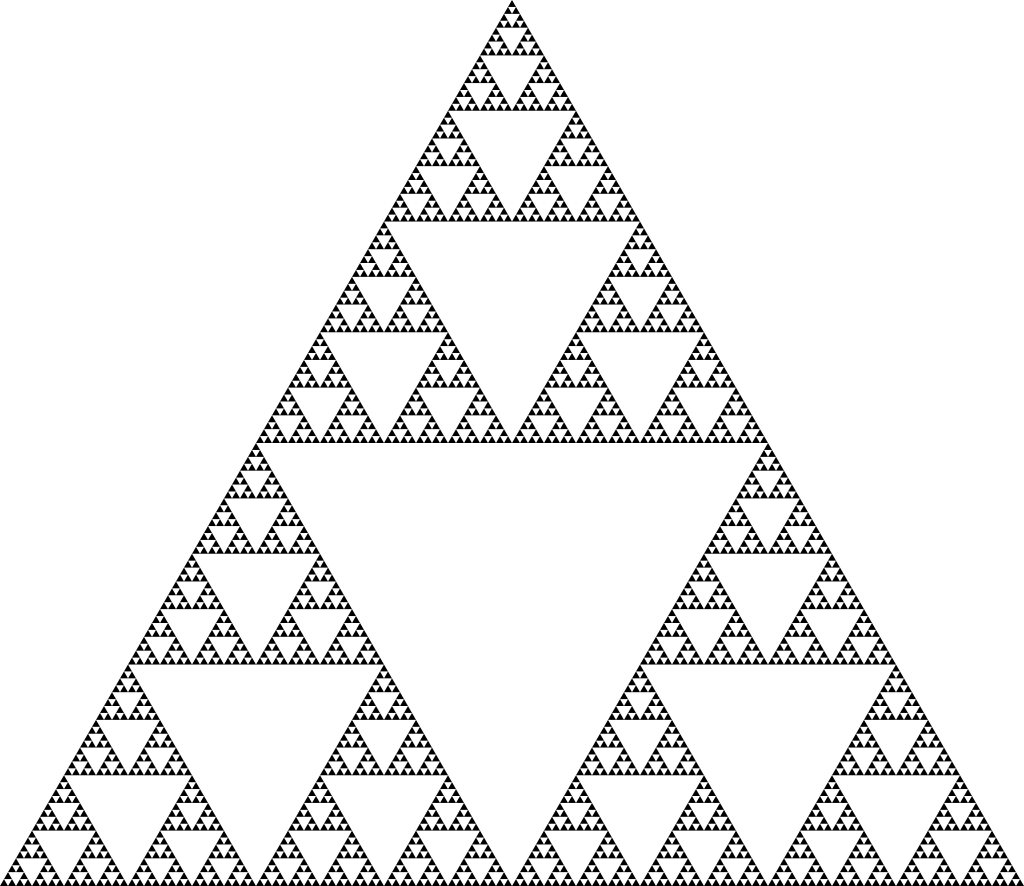
\includegraphics[scale=0.4]{sier.png}
    \\[2cm]
    \vfill
    % Bottom of the page
     \large Pierre \textsc{Thiebeaux} \\
    {\large Année scolaire 2019 - 2020}

  \end{center}
  \end{sffamily}
\end{titlepage}
\pagestyle{empty}
\tableofcontents
%\end{tikzpicture} 
%\end{center} 
%\dominitoc % <-- Ne pas oublier cette ligne !
\chapter{Fonctions et courbes représentatives}
\textit{C'est au XIV\up{ème} siècle que Nicolas Oresme a introduit la notion de fonction, il cherche à comprendre des phénomènes physiques, notamment la chaleur, la vitesse et établi, à l'aide d'une des premières représentations graphiques, une relation entre le temps et la vitesse.}
% http://vivienfrederic.free.fr/QuelquesReperesHistoriquesLesfonctions.pdf




\section{Définitions et notations}


\begin{defn}
Une fonction $f$, est un procédé qui, à un nombre \underline{de départ} lui associe un \underline{unique} nombre d'arrivé, appelé \underline{image}.

%Une fonction est la donnée d'un ensemble de nombre noté $D_f$, appelé ensemble de définition et d'un objet $f:x \rightarrow f(x)$ qui à n'importe quel nombre $x$ de $D_f$ lui associe un \underline{unique} nombre noté $f(x)$, appelé image de $x$ par $f$.
\end{defn}

\underline{Exemple}: Soit Julien un individu de 35 ans, on peut faire la fonction ($f$) qui à l'âge de Julien lui associe sa taille, si à 17 ans Julien mesure $1,75m$, on peut écrire $f(17)=1,75$ ou encore  $f:17 \mapsto 1,75$.
 
\underline{Inversement}, si l'on a $f(25)=1,80 $ ou encore $f:25 \mapsto 1,80$, on peut traduire ceci par la phrase suivante: "À 25 ans, Julien mesurait 1,80m.". \\


On peut aussi faire la fonction ($g$) qui associe l'heure de la journée au pourcentage de la batterie d'un smartphone, si à 3h le téléphone indique 55\% de batterie on pourra écrire $g(3)=55$ ou encore $g:3 \mapsto 55$.
\underline{Inversement}, si on lit $g(7)=100$, on peut traduire ceci par la phrase suivante: "À 7h la batterie du téléphone était rechargée au maximum de sa capacité".

\begin{defn}
On appelle ensemble de définition de $f$, l'ensemble des nombres de départ, que l'on notera $D_f$.
\vspace{4mm}

\end{defn}

\underline{Exemple}: Ici pour notre premier exemple $D_f$ serai $[0;35]$ et pour notre second exemple $[0;24]$.\\ \emph{Attention cependant à la conversion temps-unité}\\

%\underline{Exemple}: Soit ici $D_f=\mathbb{R}$ et $f:x \rightarrow 2x+3$ que l'on notera aussi $f(x)=2x+3$ qui est l'image de $x$ par $f$.

%\begin{defn}
%Quand un tel nombre $f(x)$ existe, on dit que $x$ est \underline{un} antécédent de $f(x)$, attention contrairement à l'image, il n'y a \underline{pas nécéssairement unicité} de l'antécédent.
%\end{defn}

%\underline{Exemple}: Soit ici $D_f=\mathbb{R}$ et $f(x)=(x-2)(x-3)$ alors ici on $f(2)=0$ et $f(3)=0$ ainsi $3$ est \underline{un} antécédent de $0$ par $f$ et \underline{les} antécédents de $0$ par $f$ sont $2$ et $3$.


On peut donner de manière équivalente la définition d'une fonction avec des représentations graphiques, c'est ce que l'on étudiera dans la suite de ce chapitre.

\newpage

\section{Définition d'une fonction par représentation graphique}

\begin{defn}
Un point $A$ du plan est la donnée de deux nombres: son \underline{abscisse} noté $x_A$ et son \underline{ordonnée} $y_A$. Un point $A$ sera noté sous la forme suivante, $A=(x_A;y_A)$.
\end{defn}

Soit une fonction $f$ définie sur un ensemble $D_f$.

\begin{defn}

La courbe représentative de la fonction $f$, notée $C_f$,  est l’ensemble des points de coordonnées $(x ; f(x))$, avec $x$ qui prend \emph{(une par une)} toutes les valeurs de l'ensemble $D_f$.

%est le nombre de départ et $y$ l'image \textit{(le nombre d'arrivé)}, et où $x$ prend toutes les valeurs de l’ensemble $D_f$. 

%On note parfois $C_f$, $\{y=f(x)\}$ que l'on peut traduire littéralement par:  "$y$ est l'image du nombre de départ $x$ par la fonction $f$." 

%Une fonction $f$ est la donnée d'une courbe qui se situera au dessus ou en dessous des nombres de $D_f$ représenté sur l'axe des abscisse, l'unique point au dessus ou en dessous d'un nombre de $D_f$ est appelé de ce nombre par la fonction $f$. 

%On placera les nombres de $D_f$ sur l'axe des abscisses,  l'unique po au dessus ou en dessous d'un nombre de $D_f$ est appelé image de ce nombre par la fonction $f$.

%$f:x \rightarrow f(x)$ qui à n'importe quel nombre $x$ de $D_f$ lui associe un \underline{unique} nombre noté $f(x)$, appelé image de $x$ par $f$.
\end{defn}

%Pour des questions pratiques, on travaillera ici dans un %repère orthonormé.

%L'axe des abscisses représentera les éventuels nombres réels $D_f$ et l'axe des ordonnées représentera les éventuelles valeurs prises par la fonction $f$.


\underline{Exemple}: Voici une représentation graphique d'une fonction $f$ où $D_f$ est l'intervalle $[0;5]$.
\begin{center}
\begin{tikzpicture}
\begin{axis}[
xlabel=axe des abscisses,
ylabel=axe des ordonnées,
width=9cm,height=9cm,
axis lines=left,
scaled ticks=false,
]
\addplot [red,domain=0:5]{(-((x-3)^2)+9)/3};
\end{axis}
\node[right] at (7,6.5) {$C_f$};
\end{tikzpicture}
\end{center}

\subsection{L'image d'une valeur par une fonction}
Ici on se pose la question suivante: "Soit un certain nombre $a$ de $D_f$ que vaut l'image de ce nombre par $f$?".%$f(a)$?".

%\underline{Exemple}: On reprend l'exemple précédent, on pose ici $D_f=[0;5]$, $f(x)=x^2$ et $x=2$ alors ici $f(x)=2^2:=2\times 2=4$, ainsi on à pu déduire que $f(x)=4$. 

\subsubsection{Comment déterminer graphiquement l'image d'une valeur $a$ de $D_f$ par la fonction $f$?}
Voici la marche à suivre, tout d'abord il nous faut, avant de se lancer dans une éventuelle recherche: 
\begin{itemize}
\item[$\bullet$] {une représentation graphique de la fonction $f$}
\item[$\bullet$]  {la valeur $a$ de $D_f$ que l'on recherche à évaluer}
\item[$\bullet$]  {une règle.}
\end{itemize}

\underline{Exemple}: on prend la représentation graphique de la fonction suivante que l'on appelera courbe, et $a=1$ dans un premier temps et puis pour $a=3$ dans un second.


\begin{center}
\begin{tikzpicture}
\draw [dashed] (0,0) -- (,0) ;
\draw[->] (-1,0) -- (7,0);
\draw (7,0) node[right] {$x$};
\draw [->] (0,-2) -- (0,2);
\draw (0,2) node[above] {$y$};
\draw [red,domain=0:6.28,samples=100] plot({\x},{cos(((\x))*180/3)});
\foreach \x in {1,...,6} {
  \draw (\x,0.1cm) -- (\x,-0.1cm) node[below] {$\x\strut$};
}
\foreach \y in {-2,-1,1} {
  \draw (0.1cm,\y) -- (-0.1cm,\y) node[left] {$\y\strut$};
}
\node[left] at (0,2) {2};
\node[below left=0.10cm] at (0,0) {0};
%\node[above] at (3.14,0) {$\pi$};

\draw[blue] (1,0) -- (1,0.5);
\draw[olivine] (3,0) -- (3,-1);
\draw[<-,black,dashed] (0,0.5)--(1,0.5);
\draw[<-,brown,dashed] (0,-1) -- (3,-1);
\end{tikzpicture}
\end{center}

%Il suffit ensuite de tracer la droite perpendiculaire à la droite parallèle à l'axe des ordonées, passant par le point d'intersection entre la courbe et la droite $x=a$, puis de repérer le point d'intersection entre cette nouvelle droite et l'axe des ordonées, le nombre correspondant sur l'axe des ordonées sera l'image de $a$ par $f$. 

%Il suffit de partir de la valeur $a$ à évaluer sur l'axe des abscisses, de monter ou descendre jusqu'à croiser la courbe, poser la règle entre ces deux points et tout en gardant un doigt sur la courbe, faire glisser horizontalement la règle pour lire la valeur sur l'axe des ordonnées.

Il suffit de partir de la valeur $a$ à évaluer sur l'axe des abscisses. Tracer la droite verticale (donc parallèle à l'axe des ordonnées) et passant par $a$. Repérer le point où cette droite intersecte la courbe. Notre but est alors de trouver l'ordonnée de ce point. Il nous faut tracer la droite horizontale (donc parallèle à l'axe des abscisses) et passant par notre point. En regardant où elle coupe l'axe des ordonnées on peut enfin lire la valeur recherchée.

Ici on a l'image de $1$ par $f$ \textit{(en bleu)} qui est $0.5$ et de $3$ par $f$ qui est $-1$ \textit{(en vert)}.



\subsection{Les antécédents d'une valeur par une fonction}

Ici on se pose la question suivante "On se donne un certain nombre $k \in  \mathbb{R}$, quels sont les éventuels nombres de $D_f$ tel que leur image par $f$ donne $k$?". On appelera un tel nombre, s'il existe, \underline{antécédent} de $k$ par $f$.\\


%\underline{Exemple}: On reprend l'exemple précédent, on pose ici $D_f=[0;	5]$, $f(x)=x^2$ et $k=4$, on aura alors un unique antécédent qui est $2$ .

\underline{Exemple}: On reprend l'exemple précédent et l'on remarque que $1$ est antécédent de $0,5$, pour autant ce n'est pas le seul, $5$ est  aussi un antécédent de $0,5$.

On voit aussi que 3 est l'unique antécédent de -1 ici.
%\begin{center}
%\begin{tikzpicture}
%\draw [dashed] (0,0) -- (,0) ;
%\draw[->] (-1,0) -- (7,0);
%\draw (7,0) node[right] {$x$};
%\draw [->] (0,-2) -- (0,2);
%\draw (0,2) node[above] {$y$};
%\draw [red,domain=0:6.28,samples=100] plot({\x},{cos(((\x))*180/3)});
%\foreach \x in {1,...,6} {
%  \draw (\x,0.1cm) -- (\x,-0.1cm) node[below] {$\x\strut$};
%}
%\foreach \y in {-2,-1,1} {
%  \draw (0.1cm,\y) -- (-0.1cm,\y) node[left] {$\y\strut$};
%}
%\node[left] at (0,2) {2};
%\node[below left=0.10cm] at (0,0) {0};
%\node[above] at (3.14,0) {$\pi$};

%\draw[blue] (1,0) -- (1,0.5);
%\draw[olivine] (3,0) -- (3,-1);
%\draw[black,dashed] (0,0.5)--(1,0.5);
%\draw[brown,dashed] (0,-1) -- (3,-1);
%\end{tikzpicture}
%\end{center}

%\textit{Attention, les antécédents d'une fonction peuvent changer si $D_f$ est changer, il est bon d'avoir en tête l'exemple suivant: si l'on avait choisi $D_f=\mathbb{R}$ et $f(x)=x^2$ ici, il y aurait eu deux antécédents, $2$ et $-2$.}


\subsubsection{Comment déterminer graphiquement les éventuels antécédents d'une valeur $k$ prise par la fonction $f$ ?"}

Voici la marche à suivre, tout d'abord voici ce qu'il nous faut avant de se lancer dans une éventuelle recherche: 
\begin{itemize}
\item[$\bullet$] {une représentation graphique de la fonction $f$}
\item[$\bullet$]  {la valeur de $k$}
\item[$\bullet$]  {une règle.}
\end{itemize}




\underline{Exemple}: on prend la représentation graphique de la fonction suivante que l'on appelera courbe, et dans un premier temps on prendra $k=0.5$ puis $k=-1$ dans un second. 

%\begin{center}
%\begin{tikzpicture}
%\begin{axis}[
%xlabel=axe des abscisses,
%ylabel=axe des ordonnées,
%width=7cm,height=7cm,
%axis lines=left,
%scaled ticks=false,
%]
%\addplot [red,domain=0:6.28,samples=100]{cos(((\x))*180/pi)};
%\addplot [blue,domain=0:6.28]{0.5};
%\end{axis}
%\draw[brown,dashed] (1.047,0) -- (1.047,0.5);
%\end{tikzpicture}
%\end{center}


\begin{center}
\begin{tikzpicture}
\draw [dashed] (0,0) -- (,0) ;
\draw[->] (-1,0) -- (7,0);
\draw (7,0) node[right] {$x$};
\draw [->] (0,-2) -- (0,2);
\draw (0,2) node[above] {$y$};
\draw [red,domain=0:6.28,samples=100] plot({\x},{sin(((\x))*180/3)});
\foreach \x in {1,...,6} {
  \draw (\x,0.1cm) -- (\x,-0.1cm) node[below] {$\x\strut$};
}
\foreach \y in {-2,-1,1} {
  \draw (0.1cm,\y) -- (-0.1cm,\y) node[left] {$\y\strut$};
}
\node[left] at (0,2) {2};
\node[below left=0.10cm] at (0,0) {0};
%\node[above] at (3.14,0) {$\pi$};

\draw[blue] (0,0.5) -- (2.5,0.5);
\draw[olivine] (0,-1) -- (4.5,-1);
\draw[->,magenta,dashed] (2.5,0.5) -- (2.5,0);
\draw[->,black,dashed] (0.5,0.5)--(0.5,0);
\draw[brown,dashed] (4.5,0) -- (4.5,-1);
\end{tikzpicture}
\end{center}

%Il suffit ensuite de tracer la droite parallèle à l'axe des ordonnées, passant par le point d'intersection entre la courbe et la droite $y=k$, puis de repérer le point d'intersection entre cette nouvelle droite et l'axe des abscisses, le nombre correspondant sur l'axe des abscisses sera \underline{un} antécédent.

Il suffit de partir de la valeur $k$ recherchée sur l'axe des ordonnées, d'aller à droite ou à gauche jusqu'à croiser la courbe, poser la règle entre ces deux points et tout en gardant un doigt sur la courbe, faire glisser verticalement la règle pour lire la valeur sur l'axe des abscisses.

Pour trouver \underline{tous les antécédents}, il suffit de le reproduire pour chaque points d'intersection entre la droite parralèle à l'axe des abscisses et passant par $k$, (\emph{notée souvent $y=k$}), et la courbe.



\section{Appartenance d'un point à une courbe}

On dit qu'un point $A$ appartient à une courbe $\mathcal{C}_f$ si jamais le point se trouve sur la représentation graphique, on notera $A \in \mathcal{C}_f$.

\underline{Exemple}: Soit ici $A=(0,75;0,7)$ et la représentation graphique précédente alors on dit que $A$ appartient à la courbe contrairement à $B=(1,5;0,7)$.

\begin{center}
\begin{tikzpicture}
\draw [dashed] (0,0) -- (,0) ;
\draw[->] (-1,0) -- (7,0);
\draw (7,0) node[right] {$x$};
\draw [->] (0,-2) -- (0,2);
\draw (0,2) node[above] {$y$};
\draw [red,domain=0:6.28,samples=100] plot({\x},{sin(((\x))*180/3)});
\foreach \x in {1,...,6} {
  \draw (\x,0.1cm) -- (\x,-0.1cm) node[below] {$\x\strut$};
}
\foreach \y in {-2,-1,1} {
  \draw (0.1cm,\y) -- (-0.1cm,\y) node[left] {$\y\strut$};
}
\node[left] at (0,2) {2};
\node[below left=0.10cm] at (0,0) {0};
\node[orange] at (0.75,0.707) {$\bullet$} ;
\node[below right=0.05cm,orange] at (0.75,0.707) {$A$};
\node[blue] at (1.5,0.707) {$\bullet$} ;
\node[below right=0.05cm,blue] at (1.5,0.707) {$B$};
%\node[above] at (3.14,0) {$\pi$};

%\draw[blue] (0,0.5) -- (0.523,0.5);
%\draw[olivine] (0,-1) -- (4.712,-1);
%\draw[black,dashed] (0.523,0)--(0.523,0.5);
%\draw[brown,dashed] (4.712,0) -- (4.712,-1);
\end{tikzpicture}
\end{center}

\begin{prop}
Un point $A=(x_A;y_A)$ appartient à une courbe $\mathcal{C}_f$ représentant une fonction $f$ si et seulement si $x_A \in D_f$ et $f(x_A)=y_A$.
\end{prop}

\section{Variation de fonction}
\begin{defn}
On dit qu'une fonction $f$ est \underline{croissante} sur un intervalle $I$ inclus dans $D_f$ si elle respecte l'ordre sur $I$, c'est à dire que pour tout nombre $x_1,x_2\in I$ tels que $x_1 \leq x_2$ alors $f(x_1) \leq f(x_2)$. %la courbe de cette fonction \underline{monte} sur cet intervalle $I$. 
\end{defn}

\begin{defn}
On dit qu'une fonction $f$ est \underline{décroissante} sur un intervalle $I$ inclus dans $D_f$ si elle change l'ordre sur $I$, c'est à dire que pour tout nombre $x_1,x_2\in I$ tels que $x_1 \leq x_2$ alors $f(x_1) \geq f(x_2)$. %la courbe de cette fonction \underline{monte} sur cet intervalle $I$. %la courbe de cette fonction \underline{descend} sur cet intervalle $I$. 
\end{defn}

Pour décrire ce phénomène on fait appel à un tableau appelé tableau de variation.

\underline{Exemple}: on reprend l'exemple précédent, voici son tableau de variation .

\begin{center}
\begin{tikzpicture}
   \tkzTabInit{$x$ / 1 , $f(x)$ / 2}{$0$, $1{,}5$, $4{,}5$,$6$}
   \tkzTabVar{-/ 0, +/ $f(1{,}5)=1$, -/ -1, +/0 }
\end{tikzpicture}
\end{center}


%En particulier, l'une des applications principales de l'étude de variation est de savoir s'il y a conservation de l'ordre, on en reparlera plus tard dans le chapitre dans la partie inéquation, une autre application est l'étude d'extrema.


\section{Extrema}
On est souvent amené à chercher les extremas d'une fonction $f$, un extrema correspond à un minimum ou à un maximum prise par au moins une valeur de $f$. Dans une représentation graphique, ces extremas sont donnés par les ordonnées des points de la courbe les plus hauts \underline{et} les plus bas.\\

Pour trouver en quelle valeur est atteint un extréma on applique la recherche d'antécédents.

\begin{center} 
\begin{tikzpicture} 
%\draw [red,domain=0:1.5]{x^3+1}; 
%\draw [blue,domain=1.5:3.337] plot({\x},%(\x-1.5)^2+(1.5)^3+1}); 
%\draw [brown,domain=3.337:5]{1}; 
%\draw [black,domain=0:1.5]{0}; 
%\draw [dashed] (-1,0) -- (6,0) ;
\draw[->] (-1,0) -- (5,0);
\draw (5,0) node[right] {$x$};
\draw [->] (0,-2) -- (0,6);
\draw (0,6) node[above] {$y$};
\foreach \x in {1,...,5} {
  \draw (\x,0.1cm) -- (\x,-0.1cm) node[below] {$\x\strut$};
}
%\foreach \y in {-2,...,6} {
  %\draw (0.1cm,\y) -- (-0.1cm,\y) node[below left=0.03cm]
  %\draw (0.1cm,\y) -- (-0.1cm,\y) node[below left=0.03cm] {$\y\strut$};
  
\foreach \y in {-2,-1.75,...,6} {
  %\draw (0.1cm,\y) -- (-0.1cm,\y) node[below left=0.03cm]
  \draw (0.1cm,\y) -- (-0.1cm,\y) node[below left=0.03cm] {$ \strut$};
}

\foreach \y in {-2,...,6} {
\draw (0.1cm,\y) -- (-0.1cm,\y) node[left =0.05cm] {$\y$};
}
  

%\draw [red,domain=0:1.5] plot({\x},\x^3+1);
%\draw [blue,domain=1.5:3.4685]plot(\x,{-(\x-1.5)^2+(1.5)^3+1});
%\draw [brown,domain=3.4685:5] plot(\x,0.5);
\draw [red,domain=1.1:4.6,smooth] plot(\x,{(\x-1)*(\x-3)*(\x-4)+2});
\node[red] at (1.1,2.551) {$\bullet$} ;
\node[red] at (4.6,5.540) {$c$} ;
\node[red] at (4.6,3) {$C_f$} ;
\end{tikzpicture} 
\end{center} 

 
Ici il y a un maximum de $5,5$ atteint en une unique valeur de $4,6$ et un minimum de $1,25$ atteint en une unique valeur de $3,6$. Attention, il n'existe pas forcément une unique valeur qui atteint un extréma.\\


Si nous sommes en possession d'un tableau de variation complet, il est possible de déterminer les extremas de la fonction sans même en avoir une représentation graphique.\\

\begin{defn}
$f$ admet un \underline{maximum} en $x=a$ si et seulement si pour tout $x\in D_f$ on a $f(x)\leq f(a)$.

$f$ admet un \underline{minimum} en $x=a$ si et seulement si pour tout $x\in D_f$ on a $f(x)\geq f(a)$.

\vspace{2mm}
\end{defn}

\underline{Exemple}: Voici la représentation graphique et le tableau de variation de notre exemple précédent.

\begin{center}
\begin{tikzpicture}
\draw [dashed] (0,0) -- (,0) ;
\draw[->] (-1,0) -- (7,0);
\draw (7,0) node[right] {$x$};
\draw [->] (0,-2) -- (0,2);
\draw (0,2) node[above] {$y$};
\draw [red,domain=0:6.28,samples=100] plot({\x},{sin(((\x))*180/3)});
\foreach \x in {1,...,6} {
  \draw (\x,0.1cm) -- (\x,-0.1cm) node[below] {$\x\strut$};
}
\foreach \y in {-2,-1,1} {
  \draw (0.1cm,\y) -- (-0.1cm,\y) node[left] {$\y\strut$};
}
\node[left] at (0,2) {2};
\node[below left=0.10cm] at (0,0) {0};
%\node[above] at (3.14,0) {$\pi$};

\draw[blue] (0,1) -- (1.5,1);
\draw[olivine] (0,-1) -- (4.5,-1);
%\draw[magenta,dashed] (2.5,0) -- (2.5,0.5);
\draw[black,dashed] (1.5,0)--(1.5,1);
\draw[brown,dashed] (4.5,0) -- (4.5,-1);
\end{tikzpicture}
\end{center}


\begin{center}
\begin{tikzpicture}
   \tkzTabInit{$x$ / 1 , $f(x)$ / 2}{$0$, $1.5$, $4.5$,$6$}
   \tkzTabVar{-/ 0, +/ 1, -/ -1, +/0 }
\end{tikzpicture}
\end{center}

Cette fonction admet pour extrema 1 et -1, le maximum 1 est atteint en 1,5 et le minimum -1 est atteint en 4,5.

\section{Résolution graphique d'équations du type $f(x)=k$, $f(x)\geq k$ et $f(x) > k$}
\subsection{Résoudre une équation du type $f(x)=k$}

\begin{center}
\begin{tikzpicture}[scale=1.7]
\draw [dashed] (0,0) -- (,0) ;
\draw[->] (-1,0) -- (7,0);
\draw (7,0) node[right] {$x$};
\draw [->] (0,-2) -- (0,2);
\draw (0,2) node[above] {$y$};
%\draw [red,domain=0:6.28,samples=100] plot({\x},{sin(((\x))*180/3)});
\draw[color=red,smooth,samples=100,domain=0:5.1] plot(\x,{0-(\x/1.3)*((\x/1.3)-2)^(2)*((\x/1.3)-4)-2});
\draw[,dashed,color=black,smooth,samples=100,domain=0:6] plot(\x,{1});
\foreach \x in {1,...,6} {
  \draw (\x,0.1cm) -- (\x,-0.1cm) node[below] {$\x\strut$};
}
\foreach \y in {-2,-1,1} {
  \draw (0.1cm,\y) -- (-0.1cm,\y) node[left] {$\y\strut$};
}
\node[left] at (0,2) {2};
\node[below left=0.10cm] at (0,0) {0};
\node[above] at (5.3,-0.7) {$C_f$};
\node[above] at (6,1) {$y=k$};
%\draw[blue] (0,1) -- (1.5,1);
%\draw[olivine] (0,-1) -- (4.5,-1);
%\draw[magenta,dashed] (2.5,0) -- (2.5,0.5);
%\draw[black,dashed] (1.5,0)--(1.5,1);
%\draw[brown,dashed] (4.5,0) -- (4.5,-1);
\end{tikzpicture}
\end{center}


Résoudre une équation du type $f(x)=k$ c'est déterminer \underline{l'ensemble des solutions} $S\subset D_f$ constitué de \underline{tous} les éléments $x\in D_f$ tel que $f(x)=k$.

\subsubsection{Méthode de résolution graphique d'équations du type $f(x)=k$}
Ici on obtiendra l'ensemble $S$ en pratiquant la méthode de recherche d'antécédents, $S$ sera l'ensemble de  \underline{tous} les antécédents de $k$ par $f$.

\subsection{Résoudre une inéquation du type $f(x)\geq k$}
Résoudre une inéquation du type $f(x) \geq k$ c'est déterminer \underline{l'ensemble des solutions} $S\subset D_f$ constitué de \underline{tous} les éléments $x\in D_f$ tel que $f(x)\geq k$.
\subsubsection{Méthode de résolution graphique d'inéquations du type $f(x)\geq k$}
On trace ici la droite $y=k$ sur la représentation graphique puis l'on cherche l'ensemble des points de la courbe $C_f$ situés \underline{au-dessus} de cette droite. Les solutions sont tous les nombres qui sont abscisses de ces points. L'ensemble $S$ est une union d'intervalle.

Le cas \underline{d'inégalité stricte} se traite presque de la même façon, la différence est l'exclusion  de l'ensemble des solutions de $f(x)=k$.

%\subsubsection{Méthode de résolution graphique d'inéquation du type $f(x) > k$}
%On trace ici la droite $y=k$ sur la représentation graphique puis l'on cherche l'ensemble des points %\underline{strictement au dessus} de cette droite. Les solutions sont les abscisses de ces points. 
%L'ensemble $S$ est une union d'intervalle.

\section{Dresser le tableau de signe d'une fonction avec une représentation graphique}
On cherche ici à savoir quand une fonction $f$ est positive ou négative ce qui revient à résoudre l'inéquation $f(x) \geq 0$, c'est à dire à remplacer $k$ par 0 et inutile de tracer la droite $y=0$ puisqu'elle est déjà représentée par l'axe des abscisses.

\begin{center}
\begin{tikzpicture}
\draw [dashed] (0,0) -- (,0) ;
\draw[->] (-1,0) -- (7,0);
\draw (7,0) node[right] {$x$};
\draw [->] (0,-2) -- (0,2);
\draw (0,2) node[above] {$y$};
\draw [red,domain=0:6.28,samples=100] plot({\x},{sin(((\x))*180/3)});
\foreach \x in {1,...,6} {
  \draw (\x,0.1cm) -- (\x,-0.1cm) node[below] {$\x\strut$};
}
\foreach \y in {-2,-1,1} {
  \draw (0.1cm,\y) -- (-0.1cm,\y) node[left] {$\y\strut$};
}
\node[left] at (0,2) {2};
\node[below left=0.10cm] at (0,0) {0};
%\node[orange] at (0.75,0.707) {$\bullet$} ;
%\node[below right=0.05cm,orange] at (0.75,0.707) {$A$};
%\node[blue] at (1.5,0.707) {$\bullet$} ;
%\node[below right=0.05cm,blue] at (1.5,0.707) {$B$};
%\node[above] at (3.14,0) {$\pi$};

%\draw[blue] (0,0.5) -- (0.523,0.5);
%\draw[olivine] (0,-1) -- (4.712,-1);
%\draw[black,dashed] (0.523,0)--(0.523,0.5);
%\draw[brown,dashed] (4.712,0) -- (4.712,-1);
\end{tikzpicture}
\end{center}



Par suite on dresse un tableau de signe.
\begin{center}
\begin{tikzpicture}
   \tkzTabInit{$x$ / 1 , $f(x)$ / 1}{$0$, $3$, $6$}
   \tkzTabLine{, +, z, -}
\end{tikzpicture}
\end{center}


\begin{comment}
\section{Équations, inéquations}
\subsection{Équations}
\begin{defn}
Une équation $E$ est une égalité mathématique qui peut faire intervenir des variables et qui n'est pas nécéssairement vrai. \\

\underline{Résoudre une équation}, c'est trouver \underline{toutes} les valeurs des variables possibles tel que l'égalité deviennent vrai. Si l'on met \underline{toutes} ces valeurs dans un même ensemble on obtient alors \underline{l'ensemble des solutions} associé à l'équation $E$, que l'on notera $S$. 
\end{defn}

\subsubsection{Équation du premier degré}
Ici on se donne une variable réelle que l'on note $x$, une équation du premier degré est une égalité du type: 
$$(E) \; ax+b=0 $$ 
où $a\in \mathbb{R}^{*}$ et $b\in \mathbb{R}$.

Notre but est de résoudre ce type d'équation, dans une équation du premier degré on peut décrire directement l'ensemble des solutions $S$.

$$S=\{ - \frac{b}{a}\}$$
On remarque que ce type d'équation admet toujours une \underline{unique} solution.\\


\underline{Exemple}: On souhaite résoudre l'équation suivante, $(E) \; 4x+3=0$, cette équation n'est pas vrai par exemple pour $x=0$ ou encore pour $x=2$.

Il nous faut donc trouver l'ensemble des solutions $S$ pour savoir pour quel valeur de $x$ l'équation $E$ est vrai. Ici $S=\{-\frac{3}{4}\}$, donc l'équation $E$ est vrai si et seulement si $x\in S$ ou encore ici, $x=-\frac{3}{4}$.


\subsection{Inéquations}
\begin{defn}
Une inéquation $I$ est une inégalité mathématique qui peut faire intervenir des variables et qui n'est pas nécéssairement vrai. \\

\underline{Résoudre une inéquation}, c'est trouver \underline{toutes} les valeurs des variables possible tel que l'inégalité soit vrai. Si l'on met \underline{toutes} ces valeurs dans un même ensemble on obtient alors \underline{l'ensemble des solutions} associé à l'inéquation $I$, que l'on notera aussi $S$. 
\end{defn}

\subsubsection{Inéquation du premier degré}

Une différence notable entre la résolution d'inéquation et la résolution d'équations se trouve dans le  \underline{signe des nombres}, qui doit être prise en compte dans les inéquations contrairement au équations donc il n'y aura pas de méthode générale ici.\\


\underline{Exemple}: Résolvons l'inéquation suivante:
$$(I) \; -3x+2\leq 0$$
$$(I) \; -3x\leq -2$$
$$(I) \; x \geq \frac{2}{3}$$

Ainsi on a $S=[\frac{2}{3};+\infty]$. On remarque le changement de signe entre la deuxième ligne et la troisième ligne qui est dû au fait que $-3$ soit négatif.

\subsubsection{Tableau de signe}
De manière analagogue au tableau de variation on peut dresser le tableau de signe d'une expression mathématique ce qui nous permettra de connaitre simplement le signe d'expression parfois plus complexe.

Voici un tableau de signe en reprenant l'exemple précédant:
\begin{center}
\begin{tikzpicture}
   \tkzTabInit{$x$ / 1 , $-3x+2$ / 1}{$-\infty$, $0$, $\frac{2}{3}$, $+\infty$}
   \tkzTabLine{, , +, , z, -, }
\end{tikzpicture}
\end{center}

l'intérêt de cet outil réside dans la résolution d'inéquation plus complexe tel que 

$$(I) \;  (-3x+2)(4x+3)\geq 0$$

Pour cela on rappel quelques règles mémotechniques: $"+ \times + donne +"$, $"- \times - donne +"$, $"- \times + donne -"$ et $"+ \times - donne -"$.  

\begin{center}
\begin{tikzpicture}
   \tkzTabInit{$x$ / 1 , $-3x+2$ / 1, $4x+3$ /1 , $(-3x+2)(4x+3)$ /1}{$-\infty$, -$\frac{3}{4}$ ,$0$, $\frac{2}{3}$, $+\infty$}
   \tkzTabLine{,+, , , +, , z , -, }
   \tkzTabLine{,-,z, , +, ,  , +, }
   \tkzTabLine{,-,z, , +, , z , -, }
\end{tikzpicture}
\end{center}

Ainsi l'ensemble des solutions est 
$ S= [-\frac{3}{4}; \frac{2}{3}] $.
\end{comment}

\section{Égalité de fonctions et interprétation graphique}

Prenons deux fonctions $(D_f,f)$ et $(D_g,g)$, on suppose qu'il existe un nombre $i$ qui appartient à $D_f$ et à $D_g$ et tel que $f(i)=g(i)$. Cette égalité est \underline{ponctuelle} (c'est à dire en \underline{un} nombre) et ce traduit graphiquement de manière intuitive grâce à une intersection de courbe, il est très facile de détecter quand deux fonctions prennent la même valeur.

\underline{Exemple}: Prenons deux fonctions réprésentées sur le même graphique %Prenons $([0;1,2],x^2)$ et $([0;1],x^3)$  et traçons leurs représentations graphiques respectives.
 
\begin{center}
\begin{tikzpicture}
\begin{axis}[
xlabel=$x$,
ylabel=$y$,
width=7cm,height=7cm,
axis lines=left,
scaled ticks=false,
]
\addplot [red,domain=0:1.2]{x^2};
\addplot [blue,domain=0:1]{x^3};
\end{axis}
\draw [dashed] (4.5,0) -- (4.5,3.8);
\node[orange] at (4.5,3.8) {$\bullet$} ;
\node[above left=0.05cm,orange] at (4.5,3.8) {$I_1$};
\node[purple] at (0,0) {$\bullet$} ;
\node[above left=0.05cm,purple] at (0,0) {$I_2$};
\end{tikzpicture}
\end{center}

Ainsi les deux courbes s'intersectent en 2 points, $I_1$ et $I_2$, on peut ainsi trouver $i_1$ en appliquant la recherche d'antécédents à la valeur $k=y_{I_1}$ ou $k=y_{I_2}$ pour trouver $i_2$.

Autrement dit, les courbes s'intersectent en $I_1$ et $I_2$ et elles sont donc égales en $x_{I_1}$ et $x_{I_2}$.

\section{Inégalité de fonctions et interprétation graphique}

Prenons les deux fonctions précédentes, on remarque que la courbe bleu est en dessous de la courbe rouge sur un intervalle, on dira alors que \underline{sur cet intervalle}, la fonction bleue est inférieure à la fonction rouge.

Attention, être inférieur ou supérieur sur un intervalle ne veut pas dire que ceci est vrai sur n'importe quel intervalle, en voici un contre-exemple.

\begin{center}
\begin{tikzpicture}
\draw [dashed] (0,0) -- (,0) ;
\draw[->] (-1,0) -- (7,0);
\draw (7,0) node[right] {$x$};
\draw [->] (0,-2) -- (0,2);
\draw (0,2) node[above] {$y$};
\draw [red,domain=0:6.28,samples=100] plot({\x},{sin(((\x))*180/pi)});
\draw [blue,domain=0:6.28,samples=100] plot({\x},{cos(((\x))*180/pi)});
\foreach \x in {1,...,6} {
  \draw (\x,0.1cm) -- (\x,-0.1cm) node[below] {$\x\strut$};
}
\foreach \y in {-2,-1,1} {
  \draw (0.1cm,\y) -- (-0.1cm,\y) node[left] {$\y\strut$};
}
\node[left] at (0,2) {2};
\node[below left=0.10cm] at (0,0) {0};
\node[orange] at (0.785,0.707) {$\bullet$} ;
\node[below right=0.05cm,orange] at (0.785,0.707) {$A$};
\node[blue] at (1.507,0.707) {$\bullet$} ;
\node[below right=0.05cm,blue] at (1.507,0.707) {$B$};
\node[above] at (3.14,0) {$\pi$};

\draw[blue] (0,0.5) -- (0.523,0.5);
\draw[olivine] (0,-1) -- (4.712,-1);
\draw[black,dashed] (0.523,0)--(0.523,0.5);
\draw[brown,dashed] (4.712,0) -- (4.712,-1);
\end{tikzpicture}
\end{center}


\chapter{Multiple, diviseur et nombre premier}

\textit{Depuis plus d'un siècle, la technologie nous permet de communiquer entre nous sans se rencontrer directement. Mais elle s'accompagne d'un défaut majeur, la sécurité.
\\
 Comment éviter que mon message soit reçu par quelqu'un d'autre que par son destinataire? \\
On a créé pour cela une matière à part entière, la cryptographie, qui a pour but de conserver une information\\ 
\vspace{2mm} confidentielle, au coeur de cette matière se trouvent les nombres premiers, qui sont indispensables.\\
En particulier on peut citer Alan Turing, un mathématicien britannique héros de guerre, qui a aidé à décrypter énigma, une machine principalement utilisée par les Allemands pour communiquer, plusieurs centaines de milliers de victimes ont pu être épargnées grâce aux messages interceptés et décryptés.}  


\section{Multiple et diviseur}
\subsection{Ensemble et appartenance}
\begin{defn}
On notera $\mathbb{N}:=\{0;1;2;3;...\}$, cet ensemble sera dit l'ensemble des entiers naturels.

On notera $\mathbb{Z}:=\{...;-3;-2;-1;0;1;2;3;...\}$, cet ensemble sera dit l'ensemble des entiers relatifs.

Si l'on note $\mathbb{N}^{*}$ ou $\mathbb{Z}^{*}$ cela signifie que l'on regarde l'ensemble sans l'élément $0$.

On dit qu'un élément $a$ appartient à un ensemble $E$ s'il fait parti des éléments qui constituent $E$, on notera $a\in E$. 
\end{defn}


\underline{Exemple}: $2\in \mathbb{N}$, ce qui se traduit en français par: deux appartient à l'ensemble des entiers naturels.


\subsection{Multiple et diviseur}

\underline{Exemple de multiple}: $8=4 \times 2$ est un multiple de $4$, $3$ est un diviseur de $99=3 \times 33$.

\begin{defn}
Soit $a,b\in \mathbb{N}$ on dit que $b$ est un multiple de $a$ s'il existe un élément $q\in \mathbb{N}$ tel que $b=aq$.

On dit que $a$ est un diviseur de $b$ s'il existe un élément $q\in \mathbb{N}$ tel que $b=aq$
\end{defn}


\begin{defn}
Pour chaque élément de $\mathbb{N}$, on peut dire s'il est pair ou impair, on dira qu'un élément $a$ est pair s'il existe un élément $q_a \in \mathbb{N}$ tel que $a=2q_{a}$, on dira que $a$ est impair s'il n'est pas pair.\\

Autrement dit, on dit qu'un nombre est pair si c'est un multiple de 2.
\end{defn}


\underline{Exemple}: 13230232 est pair, 23427865 est impair.

(Astuce, un nombre est pair si et seulement si il se termine par 0,2,4,6,8) 


\begin{prop}
Si $a$ est impair si et seulement si il existe un élément $q_{a} \in \mathbb{N}$ tel que $a=2q_{a}+1$
\end{prop}
\begin{thm}
Soit $a \in \mathbb{N}$ et $b,c$ deux multiples de $a$ alors $b+c$ est un multiple de $a$.
\end{thm}
\begin{demo}
On a $b=aq_b$ et $c=aq_c$ donc $b+c=aq_b+aq_c$ ou encore $b+c=a(q_b+q_c)$ ce qui équivaut à dire que $b+c$ est un multiple de $a$.
\end{demo}
\begin{thm}
Le carré d'un nombre impair est impair.
\end{thm}
\begin{demo}
Soit $a$ un nombre impair, par la propriété 1 on a $a=2q_{a}+1$ mais alors $a^2=(2q_{a}+1)^2$. 

On développe et l'on a $a^2=4q_{a}^2+ 4q_{a}+1$ et on factorise les deux premiers termes du second membre par $2$ pour aboutir à l'expression suivante $a^2=2( 2q_{a}^2+2q_{a} )+1$ qui équivaut à dire que $a^2$ est impair d'après la propriété 1.
\end{demo}

\section{Nombre premier}




\begin{defn}
Un nombre est dit premier s'il possède \underline{uniquement} deux diviseurs différents, qui sont nécessairement 1 et lui même.
Attention, d'après notre définition 1 n'est pas premier.
\end{defn}

\underline{Exemple de nombre}: 3 est premier, 7 et 11 sont premiers, 2 est premier, et c'est le seul nombre premier pair, ce qui est remarquable. 57 lui en revanche n'est pas premier car il est divisible par 3.

Une application très commode des nombres premiers est de réduire de manière irréductible une fraction, il est très important de savoir réduire une fraction sous sa forme irréductible, les nombres premiers serviront notamment pour montrer que certain nombres sont irrationnels dans le courant de l'année.\\


\underline{Application}: On se propose de réduire ( sous forme irréductible ) $\frac{ 337 500}{11 250}$, pour cela on décompose le numérateur et le dénominateur en produits de nombres premiers.

$337 500=2^2 \times 3^3 \times 5^5$, 


$11 250=2^1 \times 3^2 \times 5^4$

Par les règles de calcul sur les puissances on conclut que $\frac{337 500}{11 250}=30$. \\


\underline{Exemple de décomposition}: $66=3 \times 33 = 3 \times 3 \times 11 = 3^2 \times 11$ 

\begin{thm}[fondamental de l'arithmétique, admis]
Pour tout nombre $a \in \mathbb{N}$ ($\geq 2$) s'écrit comme produit de nombres premiers.
\end{thm}

\chapter{Géométrie vectorielle}

\section{Translations, vecteurs, géométrie et représentants} 

\begin{defn}
\begin{itemize}
\item Un point C est l’image d’un point D par la \underline{translation} qui transforme A en B lorsque le quadrilatère ABCD est un parallélogramme.
\item On dit alors que C est l’image du point D par la translation de \underline{vecteur} $\overrightarrow{AB}$.
\end{itemize}
\end{defn}

Translation de vecteur $\overrightarrow{AB}$ transformant C en D: 


\definecolor{ccqqqq}{rgb}{0.8,0,0}
\definecolor{qqwwwc}{rgb}{0,0.4,0.4235294117647059}
\definecolor{ududff}{rgb}{0.30196078431372547,0.30196078431372547,1}
\begin{center}


\begin{tikzpicture}[scale=1.3,line cap=round,line join=round,>=triangle 45,x=1cm,y=1cm]
\clip(-2.04154666591729,-2.509212811768067) rectangle (10.94147959627377,4.803882449981706);
\draw [->,line width=1pt,color=qqwwwc] (-1.1982293622361304,-1.1418373144650869) -- (7.648453205347327,0.5052927731930859);
\draw [->,line width=1pt,color=qqwwwc] (0.8341166330195284,2.099289632217124) -- (9.680799200602985,3.7464197198752967);
\draw [line width=1pt,dash pattern=on 1pt off 1pt,color=ccqqqq] (-1.1982293622361304,-1.1418373144650869)-- (0.8341166330195284,2.099289632217124);
\draw [line width=1pt,dash pattern=on 1pt off 1pt,color=ccqqqq] (7.648453205347326,0.5052927731930859)-- (9.680799200602985,3.7464197198752967);
\begin{scriptsize}
\draw [fill=ududff] (-1.1982293622361304,-1.1418373144650869) circle (0.5pt);
\draw[color=ududff] (-1.3721093742730635,-1.215981680182635) node {$A$};
\draw [fill=ududff] (7.648453205347326,0.5052927731930859) circle (0.5pt);
\draw[color=ududff] (7.766723955597361,0.4474685596605864) node {$B$};
\draw [fill=ududff] (0.8341166330195284,2.099289632217124) circle (0.5pt);
\draw[color=ududff] (0.9202062001450451,2.3137785848505423) node {$C$};
\draw [fill=ududff] (9.680799200602985,3.7464197198752967) circle (0.5pt);
\draw[color=ududff] (9.764892841262702,3.967085835426427) node {$D$};
\draw[color=black] (4.9202062001450451,2.6137785848505423) node {$\overrightarrow{u}$};
\draw[color=black] (3.202062001450451,-0.6) node {$\overrightarrow{u}$};
\end{scriptsize}
\end{tikzpicture}

\end{center}

% image 


\begin{rem}
\begin{itemize}
\item $(AB)$ et $(DC)$ sont parallèles (même direction),
\item AB et DC sont de même longueur,
\item $\overrightarrow{AB}$ et $\overrightarrow{DC}$ vont dans le même sens.\\
\end{itemize}
 Les vecteurs seront souvent notés $\overrightarrow{u},\overrightarrow{v},\overrightarrow{w},...$. \\
 Le vecteur $\overrightarrow{u}$ n'est pas fixe, on peut le représenter n'importe où sur une feuille, chacun de ces vecteurs est un \underline{représentant} du vecteur $\overrightarrow{u}$. 
\end{rem}

\definecolor{qqwwzz}{rgb}{0,0.4,0.6}
\begin{center}
\begin{tikzpicture}[line cap=round,line join=round,>=triangle 45,x=1cm,y=1cm]
\clip(-3.5940549442843843,-5.061970261878616) rectangle (11.456240980454272,3.847112957937895);
\draw [->,line width=1pt] (-2.3273104707114953,-3.200749924037803) -- (4.473742794457772,-1.3676535361601587);
\draw [->,line width=1pt,color=qqwwzz] (-2.2874605492358957,0.2396266300224129) -- (4.513592715933372,2.072723017900057);
\draw [->,line width=1pt,color=qqwwzz] (1.7240982126412883,-0.676921563916409) -- (8.525151477810557,1.156174823961235);
\draw [->,line width=1pt,color=qqwwzz] (3.8759939723237506,-2.7225508663305913) -- (10.677047237493017,-0.8894544784529472);
\begin{scriptsize}
\draw[color=black] (0.8790215128218503,-2.040790168612129) node {$\overrightarrow{u}$};
\draw[color=qqwwzz] (1.0149437256068465,1.3943348454086615) node {$\overrightarrow{u}$};
\draw[color=qqwwzz] (5.080253544358093,0.5293753095041458) node {$\overrightarrow{u}$};
\draw[color=qqwwzz] (7.242652384119395,-1.5218144470694197) node {$\overrightarrow{u}$};
\end{scriptsize}
\end{tikzpicture}
\end{center}

\section{Égalité de vecteurs}

\begin{defn}
Deux vecteurs $\overrightarrow{AB}$ et $\overrightarrow{DC}$ sont \underline{égaux} si et seulement si le quadrilatère ABCD est un parallélogramme (éventuellement aplati). On note alors $\overrightarrow{AB} = \overrightarrow{DC}$.
\end{defn}

Aucun des vecteurs ci-dessous ne sont égaux deux à deux.

\definecolor{qqwwzz}{rgb}{0,0.4,0.6}
\definecolor{qqwuqq}{rgb}{0,0.39215686274509803,0}
\definecolor{ccqqqq}{rgb}{0.8,0,0}
\begin{center}
\begin{tikzpicture}[line cap=round,line join=round,>=triangle 45,x=1cm,y=1cm]
\clip(-5.312960747998242,-7.95348648890992) rectangle (8.989137638993555,0.6695959841282022);
\draw [->,line width=1pt] (-2.156521746492763,-4.527209796312038) -- (3.2896341885060587,-2.8402297871782656);
\draw [->,line width=1pt,color=ccqqqq] (0.31334227843086193,-1.8237426405466266) -- (-4.814762985784294,-5.418013297066244);
\draw [->,line width=1pt,color=qqwuqq] (3.0901352292463855,-1.6551786596626903) -- (7.673510986179554,-2.8617672952563837);
\draw [->,line width=1pt,color=qqwwzz] (5.931114956424192,-3.1947109786981516) -- (0.48495902142537073,-4.881690987831924);
\begin{scriptsize}
\draw[color=black] (0.5952261336673113,-3.342947940565682) node {$\overrightarrow{u}$};
\draw[color=ccqqqq] (-2.3588673071654656,-3.3788276179847028) node {$\overrightarrow{v}$};
\draw[color=qqwuqq] (5.438982585235224,-1.9556004136968574) node {$\overrightarrow{w}$};
\draw[color=qqwwzz] (3.537359682027081,-4.120340951311143) node {$\overrightarrow{a}$};
\end{scriptsize}
\end{tikzpicture}
\end{center}

\begin{rem}
\begin{itemize}
\item $\overrightarrow{AB}=\overrightarrow{0}$ si et seulement si $A=B$,
\item si on fixe un point O, alors pour tout vecteur $\overrightarrow{u}$, il existe un unique point M vérifiant  $\overrightarrow{u}=\overrightarrow{OM}$.
\end{itemize}
\end{rem}

\section{Opposé d'un vecteur}

\begin{defn}
Quels que soient les points A et B, le vecteur $\overrightarrow{BA}$ est appelé \underline{vecteur opposé} au vecteur $\overrightarrow{AB}$, on le note aussi $-\overrightarrow{AB}$.
\end{defn}
%illustration
\definecolor{ffwwqq}{rgb}{1,0.4,0}
\definecolor{ududff}{rgb}{0.30196078431372547,0.30196078431372547,1}
\begin{center}
\begin{tikzpicture}[scale=0.7,line cap=round,line join=round,>=triangle 45,x=1cm,y=1cm]
\clip(-3.0605420727142807,-3.2026265759689405) rectangle (12.906864579078977,4.52947043231683);
\draw [->,line width=1pt] (-1.6619982425971727,-1.226011478166051) -- (2.8941761127798924,1.9885488541990934);
\draw [->,line width=1pt,color=ffwwqq] (1.7506648269583551,-0.7831880211846782) -- (8.166502184530142,0.5849926161442878);
\draw [->,line width=1pt] (7.781286276932663,4.224618777582509) -- (3.225111921555598,1.0100584452173642);
\draw [->,line width=1pt,color=ffwwqq] (11.580312124273307,-1.248103771733356) -- (5.16447476670152,-2.616284409062322);
\begin{scriptsize}
\draw[color=black] (0.32085598967479245,0.62470663307213) node {$\overrightarrow{u}$};
\draw [fill=ududff] (1.7506648269583551,-0.7831880211846782) circle (1.5pt);
\draw[color=ududff] (1.8828215920981715,-0.42232525426661893) node {$D$};
\draw [fill=ududff] (8.166502184530142,0.5849926161442878) circle (1.5pt);
\draw[color=ududff] (8.302328573486564,0.9508313192923962) node {$E$};
\draw[color=ffwwqq] (4.766450396572102,0.26425303251288856) node {$\overrightarrow{DE}$};
\draw[color=black] (5.913482283910851,2.564290293224239) node {$-\overrightarrow{u}$};
\draw[color=ffwwqq] (8.182177373300151,-1.5036860559443435) node {$\overrightarrow{ED}$};
\end{scriptsize}
\end{tikzpicture}
\end{center}

\section{Somme de deux vecteurs}
\begin{defn}
Soit $\overrightarrow{u}$ et $\overrightarrow{v}$ deux vecteurs, on définit le vecteur $\overrightarrow{w}=\overrightarrow{u}+\overrightarrow{v}$ de la façon suivante: \\

soit A un point du plan, on trace le représentant de $\overrightarrow{u}$ d'origine A : il a pour extrémité B, puis on trace le représentant de $\overrightarrow{v}$ d'origine $B$ : il a pour extrémité C.\\

La vecteur $\overrightarrow{AC}$ est un représentant du vecteur $\overrightarrow{w}$.
\end{defn}
%image 

\definecolor{wwqqcc}{rgb}{0.4,0,0.8}
\definecolor{qqqqff}{rgb}{0,0,1}
\definecolor{ffqqqq}{rgb}{1,0,0}
\definecolor{cqcqcq}{rgb}{0.7529411764705882,0.7529411764705882,0.7529411764705882}

\begin{center}
\begin{tikzpicture}[scale=1.5,line cap=round,line join=round,>=triangle 45,x=1cm,y=1cm]
\draw [color=cqcqcq,, xstep=0.5cm,ystep=0.5cm] (-0.39818369975740425,-1.7292135206977852) grid (5.432350729346309,3.3525116238702024);
\clip(-0.39818369975740425,-1.7292135206977852) rectangle (5.432350729346309,3.3525116238702024);
\draw [->,line width=0.8pt,color=ffqqqq] (1,-1) -- (5,1);
\draw [->,line width=0.8pt,color=qqqqff] (5,1) -- (3,3);
\draw [->,line width=0.8pt,dash pattern=on 1pt off 1pt,color=wwqqcc] (1,-1) -- (3,3);
\begin{scriptsize}
\draw[color=ffqqqq] (3.156842903524037,-0.05348012180948612) node {$\overrightarrow{u}$};
\draw[color=qqqqff] (4.167371937994631,2.0620878568304057) node {$\overrightarrow{v}$};
\draw[color=wwqqcc] (1.8482441538498868,1.1387987390047483) node {$\overrightarrow{w}$};
\end{scriptsize}
\end{tikzpicture}
\end{center}
\begin{prop}
Relation de Chasles: pour tout point A,B et C du plan, on a $\overrightarrow{AB} + \overrightarrow{BC} =\overrightarrow{AC}$
\end{prop}

\definecolor{wwqqcc}{rgb}{0.4,0,0.8}
\definecolor{ffqqqq}{rgb}{1,0,0}
\definecolor{qqqqff}{rgb}{0,0,1}
\definecolor{cqcqcq}{rgb}{0.7529411764705882,0.7529411764705882,0.7529411764705882}
\begin{center}

\begin{tikzpicture}[scale=1.3,line cap=round,line join=round,>=triangle 45,x=1cm,y=1cm]
\draw [color=cqcqcq,, xstep=0.5cm,ystep=0.5cm] (-0.39818369975740425,-1.7292135206977852) grid (5.432350729346309,3.3525116238702024);
\clip(-0.39818369975740425,-1.7292135206977852) rectangle (5.432350729346309,3.3525116238702024);
\draw [->,line width=0.8pt,color=ffqqqq] (1,-1) -- (5,1);
\draw [->,line width=0.8pt,color=qqqqff] (5,1) -- (3,3);
\draw [->,line width=0.8pt,dash pattern=on 1pt off 1pt,color=wwqqcc] (1,-1) -- (3,3);
\begin{scriptsize}
\draw [fill=qqqqff] (1,-1) circle (0.5pt);
\draw[color=qqqqff] (1.0485449179379063,-1.1677193438289633) node {$A$};
\draw [fill=qqqqff] (5,1) circle (0.5pt);
\draw[color=qqqqff] (5.054311090551555,1.131528745951003) node {$B$};
\draw[color=ffqqqq] (3.156842903524037,-0.15348012180948612) node {$\overrightarrow{AB}$};
\draw [fill=qqqqff] (3,3) circle (0.5pt);
\draw[color=qqqqff] (3.047793007717858,3.138046828784715) node {$C$};
\draw[color=qqqqff] (4.27371937994631,2.0620878568304057) node {$\overrightarrow{BC}$};
\draw[color=wwqqcc] (1.7582441538498868,1.1387987390047483) node {$\overrightarrow{AC}$};
\end{scriptsize}
\end{tikzpicture}
\end{center}

\begin{prop}
Quels que soient les vecteurs $ \overrightarrow{u},\overrightarrow{v}$ et $\overrightarrow{w}$ du plan, on a:
\begin{itemize}
\item $ \overrightarrow{u}+\overrightarrow{v}=\overrightarrow{v}+\overrightarrow{u}$
\item $(\overrightarrow{u}+\overrightarrow{v})+\overrightarrow{w}=\overrightarrow{u}+(\overrightarrow{v}+\overrightarrow{w})$,
\item $\overrightarrow{u}+\overrightarrow{0}=\overrightarrow{u}$
\end{itemize}
\end{prop}


\section{Différence de deux vecteurs}
\begin{defn}
Soit $\overrightarrow{u}$ et $\overrightarrow{v}$ deux vecteurs, on définit le vecteur $\overrightarrow{z}=\overrightarrow{u}-\overrightarrow{v}$ comme la somme du vecteur $\overrightarrow{u}$ et du vecteur $-\overrightarrow{v}$.
\end{defn}

\definecolor{qqwuqq}{rgb}{0,0.39215686274509803,0}
\definecolor{ccqqqq}{rgb}{0.8,0,0}
\definecolor{qqqqff}{rgb}{0,0,1}
\begin{center}
\begin{tikzpicture}[line cap=round,line join=round,>=triangle 45,x=1cm,y=1cm]
\clip(-3.056841780860057,-2.0482217238340934) rectangle (8.799310047069776,4.426348688449437);
\draw [->,line width=1pt,color=qqqqff] (-0.7864468403215852,-1.779436058074702) -- (4.779258859104043,0.27947655149801376);
\draw [->,line width=1pt,color=qqqqff] (0.4356174182635169,2.112572939375658) -- (6.001323117689145,4.1714855489483735);
\draw [->,line width=1pt,color=ccqqqq] (-0.7864468403215852,-1.779436058074702) -- (0.43561741826351685,2.112572939375658);
\draw [->,line width=1pt,color=ccqqqq] (4.779258859104043,0.2794765514980138) -- (6.001323117689145,4.1714855489483735);
\draw [->,line width=1pt,color=qqwuqq] (4.779258859104043,0.2794765514980138) -- (0.43561741826351685,2.112572939375658);
\begin{scriptsize}
\draw[color=qqqqff] (3.1305874543408243,3.337991001119945) node {$\overrightarrow{v}$};
\draw[color=ccqqqq] (5.575918768851353,2.180163674173677) node {$\overrightarrow{u}$};
\draw[color=qqwuqq] (2.913769616640166,1.3743158546190748) node {$\overrightarrow{u}-\overrightarrow{v}$};
\end{scriptsize}
\end{tikzpicture}
\end{center}


\section{Multiplication d'un vecteur par un nombre réel}

\begin{defn}
Soit $\overrightarrow{u}=\overrightarrow{AB}$ un vecteur non nul et $k \in \mathbb{R}^*$ on définit le vecteur $\overrightarrow{v}=k \overrightarrow{u} = \overrightarrow{AC}$ par :

\begin{itemize}
\item A,B et C sont alignés,
\item si $k>0$, $AC = kAB$ et B et C sont du même coté par rapport à A,
\item si $k<0$, $AC=-kAB$ et B et C sont de part et d'autre de A.
\end{itemize}
\end{defn}


\definecolor{ffvvqq}{rgb}{1,0.3333333333333333,0}
\definecolor{qqwuqq}{rgb}{0,0.39215686274509803,0}
\definecolor{zzttff}{rgb}{0.6,0.2,1}
\definecolor{cqcqcq}{rgb}{0.7529411764705882,0.7529411764705882,0.7529411764705882}

\begin{center}
\begin{tikzpicture}[scale=1.5,line cap=round,line join=round,>=triangle 45,x=1cm,y=1cm]
\draw [color=cqcqcq,, xstep=0.5cm,ystep=0.5cm] (-0.5910484495505731,-0.9956587878117392) grid (6.566912672783369,2.9132590438378);
\clip(-0.5910484495505731,-0.9956587878117392) rectangle (6.566912672783369,2.9132590438378);
\draw [->,line width=1pt] (0.5,0.5) -- (2.5,1.5);
\draw [->,line width=1pt,color=zzttff] (2,0) -- (6,2);
\draw [->,line width=1pt,color=qqwuqq] (3.5,-0.5) -- (4.5,0);
\draw [->,line width=1pt,color=ffvvqq] (6,2.5) -- (0,-0.5);
\begin{scriptsize}
\draw[color=black] (1.4389045874863182,1.0986040561836155) node {$\overrightarrow{u}$};
\draw[color=zzttff] (4.407218437093313,0.8972863996179737) node {$\overrightarrow{v}=2\overrightarrow{u}$};
\draw[color=qqwuqq] (4.5168890229519025,-0.32180385402952194) node {$\overrightarrow{w}=\frac{1}{2}\overrightarrow{u}$};
\draw[color=ffvvqq] (2.4642458265434624,1.1097883704372622) node {$\overrightarrow{x}=-3\overrightarrow{u}$};
\end{scriptsize}
\end{tikzpicture}
\end{center}

\begin{rem}
Si $\overrightarrow{u}=\overrightarrow{0}$ ou $k=0$ alors  $\overrightarrow{v}=\overrightarrow{0}$.
\end{rem}

\begin{prop}
Quels que soient les vecteurs $\overrightarrow{u}$,$\overrightarrow{v}$ et les réels $k, \lambda$ et $l$ , on a:

\begin{itemize}
\item $k(\overrightarrow{u}+\overrightarrow{v})=k\overrightarrow{u}+k\overrightarrow{v}$
\item $(k+l) \overrightarrow{u}= k\overrightarrow{u} + l \overrightarrow{u}$
\item $k(\lambda \overrightarrow{u})=(k\lambda)\overrightarrow{u}$
\item $k\overrightarrow{u}=\overrightarrow{0} \Longleftrightarrow k=0$ ou $\overrightarrow{u}=\overrightarrow{0}$.
\end{itemize}
\end{prop}
\newpage
\section{Colinéarité de deux vecteurs}

\begin{defn}
Deux vecteur $\overrightarrow{u}$ et $\overrightarrow{v}$ sont \underline{colinéaires} s'il existe $k \in \mathbb{R}^*$ tel que $\overrightarrow{v}=k\overrightarrow{u}$. \\

Autrement dit, les vecteurs $\overrightarrow{u}$ et $\overrightarrow{v}$ ont la même direction.

  
\end{defn}

\begin{prop}
\begin{itemize}
\item Trois point A,B et C sont alignés si et seulement si les vecteurs $\overrightarrow{AB}$ et $\overrightarrow{AC}$ sont colinéaires,
\item deux droites (AB) et (CD) sont parallèles si et seulement si les vecteurs $\overrightarrow{AB}$ et $\overrightarrow{CD}$ sont colinéaires.
\end{itemize}
\end{prop}

\definecolor{ttttff}{rgb}{0.2,0.2,1}
\definecolor{ffqqqq}{rgb}{1,0,0}
\definecolor{xdxdff}{rgb}{0.49019607843137253,0.49019607843137253,1}
\definecolor{ududff}{rgb}{0.30196078431372547,0.30196078431372547,1}
\begin{center}
\begin{tikzpicture}[scale=1,line cap=round,line join=round,>=triangle 45,x=1cm,y=1cm]
\clip(-3.8947407154184757,-2.0907315036595575) rectangle (13.107892447504687,5.194300200155465);
\draw [line width=0.5pt,domain=-3.8947407154184757:13.107892447504687] plot(\x,{(--0.11020359903845317--0.7172985865608171*\x)/2.165179066840997});

\draw [->,line width=1pt,color=ttttff] (-1.795978184370148,-0.5440884923310725) -- (7.018599266682028,2.3760782705941716);

\draw [->,line width=0.5pt,color=ffqqqq] (-1.795978184370148,-0.5440884923310725) -- (0.36920088247084903,0.17321009422974465);
\begin{scriptsize}
\draw [fill=ududff] (-1.795978184370148,-0.5440884923310725) circle (0.5pt);
\draw[color=ududff] (-1.6897117271018778,-0.25849738842259906) node {$A$};
\draw [fill=ududff] (0.36920088247084915,0.17321009422974462) circle (0.5pt);
\draw[color=ududff] (0.4754673397391189,0.45880119813821807) node {$B$};
\draw [fill=xdxdff] (7.018599266682028,2.3760782705941716) circle (0.5pt);
\draw[color=xdxdff] (7.130404226164512,2.6638301864548044) node {$C$};
\draw[color=ffqqqq] (-0.8528633761142532,0.11343521201634318) node {$\overrightarrow{AB}$};
\draw[color=ttttff] (2.866462628275189,1.3556495491258382) node {$\overrightarrow{AC}$};
\end{scriptsize}
\end{tikzpicture}



\definecolor{qqzzff}{rgb}{0,0.6,1}
\definecolor{ffqqqq}{rgb}{1,0,0}
\definecolor{xdxdff}{rgb}{0.49019607843137253,0.49019607843137253,1}
\definecolor{ududff}{rgb}{0.30196078431372547,0.30196078431372547,1}
\begin{tikzpicture}[scale=1.4,line cap=round,line join=round,>=triangle 45,x=1cm,y=1cm]
\clip(-3.813335559368229,-0.8053959587987695) rectangle (7.065827437128698,5.135646958819455);
\draw [line width=1pt,domain=-3.813335559368229:7.065827437128698] plot(\x,{(--11.36414460329706--2.1784623739995186*\x)/6.017338142815775});
\draw [line width=1pt,domain=-3.813335559368229:7.065827437128698] plot(\x,{(--2.8943388990546204--2.1784623739995186*\x)/6.017338142815775});
\draw [->,line width=1pt,color=ffqqqq] (-2.499993463772435,0.9834918309002973) -- (3.51734467904334,3.161954204899816);
\draw [->,line width=1pt,color=qqzzff] (2.034214551248869,1.2174484108623713) -- (3.3456860173121665,1.692241612704269);
\begin{scriptsize}
\draw [fill=ududff] (-2.499993463772435,0.9834918309002973) circle (0.5pt);
\draw[color=ududff] (-2.4279421465330735,1.1622026612707856) node {$A$};
\draw [fill=ududff] (3.51734467904334,3.161954204899816) circle (0.5pt);
\draw[color=ududff] (3.581095539813276,3.3465346066611774) node {$B$};
\draw [fill=ududff] (2.034214551248869,1.2174484108623713) circle (0.5pt);
\draw[color=ududff] (2.1022093199769754,1.400184351819155) node {$C$};
\draw [fill=xdxdff] (3.3456860173121665,1.692241612704269) circle (0.5pt);
\draw[color=xdxdff] (3.411108617993012,1.876147732915894) node {$D$};
\draw[color=ffqqqq] (0.6148237540496609,1.9271438094619733) node {$\overrightarrow{AB}$};
\draw[color=qqzzff] (2.782157007258033,1.2746863135461156) node {$\overrightarrow{CD}$};
\end{scriptsize}
\end{tikzpicture}

\end{center}


\chapter{Informations Chiffrées}

\section{Proportions et pourcentages}

    \subsection{Population et sous-population}

\begin{defn}
On appelle \underline{population} un ensemble d’éléments appelés individus.

On appelle \underline{sous-population} une partie de la population.
\end{defn}

\underline{Exemple :}  On considère une classe de seconde au sein d’un lycée. Un individu est un élève de seconde. L’ensemble des filles de cette classe de seconde constitue une sous-population des élèves de la classe.

   \subsection{Proportion d’une sous-population}

\begin{defn}
On considère une population qui possède $N$ individus et une sous-population composée de $n$ individus. La proportion d’individus de la sous-population, notée $p$, est égale à $p=\frac{n}{N}$.
\end{defn}

\underline{Exemple :}
Dans une classe, il y a 18 garçons sur les 30 élèves. La proportion de garçons dans la classe est de $\frac{18}{30}=0,6$.

\underline{Remarques :}

\begin{itemize}

\item[$\bullet$] une proportion peut être exprimée sous forme de fraction, sous forme décimale ou sous forme de pourcentage. Dans l’exemple précédent, on peut dire que $0,6 \times 100 = 60\%$ des élèves de la classe sont des garçons.

\item[$\bullet$] la proportion est un nombre toujours compris entre 0 et 1 \emph{(ou un pourcentage entre $0\%$ et $100\%$)}.
\end{itemize}

   \subsection{Proportion de proportion}

\begin{prop}
A et C sont deux sous populations d’une population E telles que C est incluse dans A. La proportion de A dans E est notée $p$ et la proportion de C dans A est notée $p’$. La proportion de C dans E est égale au produit $p\times p’$.
\end{prop}\\


\begin{center}
\definecolor{ccffww}{rgb}{0.8,1,0.4}
\definecolor{qqzzcc}{rgb}{0,0.6,0.8}
\definecolor{ffzztt}{rgb}{1,0.6,0.2}
\begin{tikzpicture}[scale=0.7,line cap=round,line join=round,>=triangle 45,x=1cm,y=1cm]
\clip(-5,-1) rectangle (2.5,3.5);
\draw [rotate around={-3.062287085400037:(-1.211512669394665,1.3886326992355753)},line width=2pt,color=ffzztt,fill=ffzztt,fill opacity=0.46] (-1.211512669394665,1.3886326992355753) ellipse (3.6966818052133736cm and 1.7935056151820508cm);
\draw [rotate around={-8.308276127483298:(-1.2181543229739313,1.5480323851379791)},line width=2pt,color=qqzzcc,fill=qqzzcc,fill opacity=0.66] (-1.2181543229739313,1.5480323851379791) ellipse (2.4514055805085846cm and 1.2405964244869365cm);
\draw [rotate around={28.570698548466485:(-1.2181543229739307,1.448407581448977)},line width=2pt,color=ccffww,fill=ccffww,fill opacity=0.75] (-1.2181543229739307,1.448407581448977) ellipse (1.117851673976015cm and 0.8161941205790404cm);
\draw (-4.359787365015315,1.6967344060660892) node[anchor=north west] {\textbf{E}};
\draw (-2.9988513562897547,2.430774623236079) node[anchor=north west] {\textbf{A}};
\draw (-1.5082773193514754,1.6813852290822337) node[anchor=north west] {\textbf{C}};
\end{tikzpicture}
\end{center}



%%%Dessin

\underline{Exemple :} On considère une entreprise qui possède des véhicules. $\frac{3}{4}$  de ces véhicules sont électriques. Parmi les véhicules électriques, la proportion de deux-roues est $0,3$.
La proportion $p$ de deux-roues électriques dans la population totale est donc : $p= \frac{3}{4} \times 0,3 =0,225$

On peut dire que les deux roues électriques représentent 22,5\% de l’ensemble des véhicules de l’entreprise.\\



\underline{Attention !} On n’effectue pas de produit avec les pourcentages ! Par exemple ici $75\% \times 30\%=2250\%$, ce qui ne représente pas une proportion. Il faut convertir sous forme décimale ou fractionnaire.
\section{Taux d'évolutions}

    \subsection{Variation absolue, variation relative}

Une quantité à une valeur de départ $V_d$. Elle varie pour atteindre une valeur d’arrivée $V_a$.

\begin{defn}
La \underline{variation absolue}, notée $\Delta V$ est donnée par $\Delta V = V_a - V_d$. \\

Le \underline{taux d’évolution} (ou évolution relative) noté $t$ est le quotient de la variation absolue $\Delta V$ par $V_d$. On a $t=\frac{\Delta V}{V_d}$. Il peut s’exprimer en pourcentage.
\end{defn}

\underline{Exemple :} Adam place 110 \euro{} en bourse. Il se rend compte 15 jours plus tard que ses actions valent 132 \euro{}. Quel est le taux d’évolution ? 

La variation absolue est $\Delta V = 132- 110=22$  . Le taux d’évolution est donc $t=\frac{22}{110}=0,2$.
On peut dire qu’il y a eu une augmentation de 20\% par rapport à la somme placée au départ.\\


\underline {Exemple :} Le prix d’une tablette tactile passe de 759 \euro{} à 683,10 \euro{}.
La variation absolue est  $\Delta V =683,10 - 759 = -75,9$   Le taux d’évolution est donc $t=-\frac{75.9}{759}=-0,1$ 
Il y a eu une réduction de 10\%.\\


\underline{Remarque :} on peut avoir une variation absolue négative, ce qui signifie que la quantité a diminué.

\begin{prop} 
Soit $t$ le taux d’évolution qui permet de passer d’une quantité $V_d$ à une quantité $V_a$. On a alors $V_a=(1+t)\times V_d$.
\end{prop}

\begin{defn}
Le nombre $1+t$ est appelé le \underline{coefficient multiplicateur}. On le note $C_m$.
\vspace{0.5cm}
\end{defn}

\underline{Remarque :} dans le cas d’une baisse, $t$ est négatif et $C_m$ est un réel compris entre $0$ et $1$. Sinon, s’il s’agit d’une augmentation, $t$ est positif et $C_m$ est supérieur à $1$.\\

\underline{Exemple :} un article à 85 \euro{} est soldé à -25\%. Quel est le nouveau prix après réduction ?
On a $V_d=85$ et $t=-0.25$ car l'article a un prix réduit de 25\%.

Calculons le coefficient multiplicateur. $C_m= V_d \times 0,75 = 85 \times 0,75 = 63,75$. Le nouveau prix de cet article est donc de 63,75 \euro{}.

\newpage

    \section{Evolutions successives} 



\begin{prop} Une valeur de départ $V_d$ subit deux évolutions successives : une évolution de coefficient multiplicateur $C_{m1}$, puis une évolution de coefficient $C_{m2}$.
Le \underline{coefficient multiplicateur global} est donné par $C_{mg}=C_{m1} \times C_{m2}$.
\end{prop}

\begin{defn}
Le taux d’évolution global, noté $T$ est $T=C_{mg}-1$
\vspace{5mm}
\end{defn}

\underline{Remarques :}
\begin{itemize}
 \item[$\bullet$] De façon équivalente, $C_{mg}=T+1$
 \item[$\bullet$] Lorsque l’on a plus de deux évolutions successives, on procède de la même manière.	
\end{itemize}

\underline{Exemple :} le nombre d’abonnés à un journal quotidien augmente de 20\% puis diminue de 10\%.  \\

Quelle est alors l’évolution globale ?\\

Augmenter de 20\% signifie que $t_1=0,2$, donc $C_{m1}=1,2$.

Diminuer de 10\% signifie que $t_2=-0,1$ donc $C_{m2}=0,9$.\\

On a alors $C_{mg} = 1,2 \times 0,9 = 1,08$. Le taux d’évolution est $T = C_{mg}-1 = 1,08-1 = 0,08$. On peut donc dire que le nombre d’abonnés a augmenté de 8\%. \\

\underline{Attention !} Lorsqu’on applique successivement des augmentations en pourcentage, le pourcentage global n’est pas la somme des pourcentages.

   \section{Evolution réciproque}
\begin{defn}
On appelle évolution réciproque l’évolution qui permet de repasser d’une quantité d’arrivé $V_a$ à une quantité de départ $V_d$. On le note $t’$.
\end{defn}

\begin{prop}
Le coefficient multiplicateur $C_{m’}$ est l’inverse du coefficient multiplicateur $C_{m}$. $C_{m’}=\frac{1}{C_m}$
\end{prop}

\underline{Exemple :} Un prix augmente de 10\%.Quelle évolution permettrait de retrouver le prix initial ?
Le coefficient multiplicateur est $C_m$=1,1. Le coefficient multiplicateur réciproque noté $C_{m’}$ est $C_{m’}=\frac{1}{1,1}\simeq 0,909$.
Le taux d’évolution réciproque est $t’=C_{m’}-1=0,909-1 \simeq - 0,091$. Il faudrait donc baisser le prix de 9.1\% pour retrouver le prix de départ et non pas de 10\% !

\chapter{Ensemble de nombre, inclusion, intervalle et distance}

\section{Ensemble de nombre, inclusion}
\subsection{Ensemble de nombre}

\subsection*{Nombres entiers naturels $\N$}

\begin{defn}
L'ensemble des  entiers naturels, noté $\mathbb{N} = \{0;1;2;3;4;\dots\}$.
C'est l'ensemble des nombres positifs  qui permettent de compter une collection d'objets.
On note $\N^*$ ou $\N-\{0\}$ l'ensemble des entiers naturels non nuls.
\end{defn}



\medskip

\underline{Exemples:}


\[245 \in \N ;\qquad -5 \notin \N ;\qquad  2^5 \in \N ;\qquad \dfrac{3}{5} \notin\N; \qquad 0 \in\N; \qquad 0 \notin\N^*\] 
La notation \og $x\in E$\fg{} signifie que l'élément $x$ \emph{appartient} à l'ensemble $E$.

 La notation \og $x\notin E$\fg{} signifie que l'élément $x$ \emph{n'appartient pas} à l'ensemble $E$.
 
\begin{comment}
\subsubsection{notions d'arithmétique}

Soient  $a$ et $b$ deux nombres entiers naturels.

\begin{itemize}
\item on dit que $b$ \emph{divise} $a$ lorsqu'il existe un entier naturel $q$ tel que $a=b\times q$. (on dit encore que $b$ est un \emph{diviseur} de $a$ ou que $a$ est un \emph{multiple} de $b$)
\item Un entier naturel $p\geqslant 2$ est un \emph{nombre premier} lorsque ses seuls diviseurs sont $1$ et $p$.
\end{itemize}
\end{comment}

\subsection*{Nombres entiers relatifs $\Z$}
\begin{defn}
L'ensemble des  nombres entiers relatifs  est $\Z=\{\dots;-2;-1;0;1;2;3;\dots\}$. Il est composé des nombres entiers naturels et de leurs opposés.

En particulier, l'ensemble $\N$ est \emph{contenu} (ou inclus) dans $\Z$, ce que l'on note \og $\N\subset \Z$\fg.
\end{defn}
 

\medskip 
La proposition \og Si $n \in \N $ alors $n\in\Z$ et $-n \in \Z $ \fg{} est vraie. 

Par contre, la réciproque \og Si $n\in\Z$ et $-n\in\Z$  alors  $n\in\N$ \fg{} est fausse. (Il suffit de choisir $n=-1$)

\underline{Exemple :}

\[245 \in \Z ;\qquad -5 \in \Z ;\qquad  2^5 \in \Z ;\qquad \dfrac{3}{5} \notin\Z; \qquad 0 \in\N; \qquad 0 \notin\Z^*\] 

\subsection*{Nombres décimaux $\D$}
\begin{defn}
Les nombres décimaux sont les nombres de la forme $\dfrac{a}{10^n}$, où $a$ est un entier et $n$ un entier naturel. 

Ce sont les nombres dont l'écriture décimale n'a qu'un nombre \emph{fini} de chiffres après la virgule.

L'ensemble des \emph{nombres décimaux} est noté  $\D$. 

\end{defn}

\medskip

\underline{Exemple :} 

\medskip

$-13 \in \D$ ; \hfill  $0,3333 \in \D$ ; \hfill $\dfrac{1}{3} \notin \D$ ; \hfill $\dfrac{3}{4} \in \D$; \hfill  $3,1416 \in \D$ ; \hfill $\pi \notin \D$.

\subsection*{Nombres rationnels $\Q$}
\begin{defn}

L'ensemble des  nombres rationnels  est $\Q=\left\{\dfrac{a}{b} \text{ où } a\in\Z,~b\in\Z^*\right\}$.

C'est l'ensemble des nombres qui s'écrivent comme le quotient d'un entier par un entier non nul.
\end{defn}

\medskip
\begin{itemize}
\item La fraction $\dfrac{a}{b}$ avec $b \ne 0$ est dite \emph{irréductible} lorsque le numérateur et le dénominateur n'ont pas de facteurs communs (autres que $1$ ou $-1$).
\item La partie décimale d'un nombre rationnel est infinie et périodique à partir d'un certain rang.
\item La division par 0 est \textbf{interdite} : l'écriture  $\dfrac{a}{0}$ n'a aucun sens.
\end{itemize}


\medskip

\underline{Exemple:}

\medskip

$-13 \in \Q$ ; \hfill  $0,5 \in \Q$ ; \hfill $-\dfrac{1}{3} \in \Q$ ; \hfill $\dfrac{22}{7} \in \Q$; \hfill  $\sqrt{2} \notin \Q$ ; \hfill $\pi \notin \Q$.

\subsection*{Nombres réels $\R$}
Dès l'antiquité, on avait découvert l'insuffisance des nombres rationnels. 

Par exemple, il n'existe pas de rationnel $x$ tel que $x^2 =2$ on dit que $\sqrt{2}$ est un irrationnel.

\underline{Exemple :}

$-13 \in \R$ ; \hfill  $0,5 \in \R$ ; \hfill $-\dfrac{1}{3} \in \R$ ; \hfill $\dfrac{22}{7} \in \R$; \hfill  $\sqrt{2} \in \R$ ; \hfill $\pi \in \R$


\medskip

\begin{defn}
L'ensemble de tous les nombres rationnels et irrationnels est l'ensemble des nombres réels noté $\R$
\vspace{0.6cm}
\end{defn}

\medskip

 Chaque nombre réel correspond à un unique point de la droite graduée. Réciproquement, à chaque point de la droite graduée correspond un unique réel, appelé \emph{abscisse} de ce point.
 
 
\vspace{3cm} 

\begin{center}
\definecolor{qqzzff}{rgb}{0,0.6,1}
\definecolor{zzccqq}{rgb}{0.6,0.8,0}
\definecolor{ffzzqq}{rgb}{1,0.6,0}
\begin{tikzpicture}[scale=2,line cap=round,line join=round,>=triangle 45,x=1cm,y=1cm]
\clip(-4.019411648148072,-0.5) rectangle (4.148615211731987,0.5);
\draw [line width=0.5pt,domain=-4.019411648148072:4.148615211731987] plot(\x,{(-0-0*\x)/4.848213562373095});
\begin{scriptsize}
\draw [fill=ffzzqq] (1.4142135623730951,0) circle (1.5pt);
\draw[color=ffzzqq] (2.153088164022291,-0.2684388991540966) node {$A = \sqrt{2}$};
\draw [fill=zzccqq] (0.3333333333333333,0) circle (1.5pt);
\draw[color=zzccqq] (0.33333333,-0.2684388991540966) node {$B = \frac{1}{3}$};
\draw [fill=qqzzff] (-3.434,0) circle (1.5pt);
\draw[color=qqzzff] (-3.43,0.2684388991540966) node {$C = -3,43$};
\draw [color=black] (0,0)-- ++(-2.5pt,0 pt) -- ++(5pt,0 pt) ++(-2.5pt,-2.5pt) -- ++(0 pt,5pt);
\draw[color=black] (0,0.36759552264277506) node {$O = 0$};
\draw [color=black] (1,0)-- ++(-2.5pt,0 pt) -- ++(5pt,0 pt) ++(-2.5pt,-2.5pt) -- ++(0 pt,5pt);
\draw[color=black] (1,0.2684388991540966) node {$U = 1$};
\draw[color=black] (4.11,0) node {$>$};
\draw[color=black] (4,-0.2) node {$\mathbb{R}$};
\end{scriptsize}
\end{tikzpicture}
\end{center}






\newpage
\subsection{Inclusions}
\begin{defn}
Soient $A$,$B$ deux ensembles, on dit que $A$ est inclu dans $B$ (on notera $A \subset B$) si tous les éléments qui appartiennent à $A$ appartiennent aussi à $B$ \vspace{1mm}

\end{defn}

Ici on a donc: 
$$\N\subset\Z\subset\D\subset\Q\subset\R$$


\definecolor{cwrbqq}{rgb}{0.7764705882352941,0.10588235294117647,0}
\definecolor{xfqqff}{rgb}{0.4980392156862745,0,1}
\definecolor{qqwwzz}{rgb}{0,0.4,0.6}
\definecolor{ttzzqq}{rgb}{0.2,0.6,0}
\definecolor{ffcctt}{rgb}{1,0.8,0.2}
\begin{center}
\begin{tikzpicture}[scale=1,line cap=round,line join=round,>=triangle 45,x=1cm,y=1cm]
\clip(-1.0852426111294717,-3.27217309615321) rectangle (13.535636833199093,6.453068116064266);
\draw [rotate around={-7.031200777095108:(6.4418004174774985,1.3825493155858697)},line width=2pt,color=cwrbqq,fill=cwrbqq,fill opacity=0.83] (6.4418004174774985,1.3825493155858697) ellipse (7.093171561653718cm and 4.436774666300759cm);
\draw [rotate around={-4.988899436588697:(5.324967336770669,1.6780180753745022)},line width=2pt,color=xfqqff,fill=xfqqff,fill opacity=0.49] (5.324967336770669,1.6780180753745022) ellipse (5.319029519842912cm and 2.9997357324987304cm);
\draw [rotate around={-3.6040220349125778:(3.80067903794055,1.8803941990661)},line width=2pt,color=qqwwzz,fill=qqwwzz,fill opacity=0.56] (3.80067903794055,1.8803941990661) ellipse (3.7363154924506854cm and 2.4076118183254493cm);
\draw [rotate around={-2.295253196636245:(3.2759884051784676,1.9667356955965696)},line width=2pt,color=ttzzqq,fill=ttzzqq,fill opacity=0.61] (3.2759884051784676,1.9667356955965696) ellipse (2.7205409136175795cm and 1.4065850757201457cm);
\draw [rotate around={-2.295253196636245:(3.2759884051784676,1.9667356955965696)},line width=2pt,color=ttzzqq,fill=ttzzqq,fill opacity=0.61] (3.2759884051784676,1.9667356955965696) ellipse (2.7205409136175795cm and 1.4065850757201457cm);
\draw [rotate around={-2.692027097027511:(2.5752852118151055,1.983538311480675)},line width=2pt,color=ffcctt,fill=ffcctt,fill opacity=0.3] (2.5752852118151055,1.983538311480675) ellipse (1.8296313805224764cm and 0.835103967296833cm);

\draw (2.1361775768797574,2.163197833290756) node[scale=1,anchor=north west] {$\mathbb{N}$};
\draw (3.4008314090388376,2.465145123109777) node[anchor=north west] {$2$};
\draw (2.0636362684117455,2.7670924129287986) node[anchor=north west] {0};
\draw (2.5381248666987783,2.5082804502267804) node[anchor=north west] {1000};
\draw (4.824297203899936,1.6887092350037232) node[anchor=north west] {-3};
\draw (5.622300755564491,1.0201116646901764) node[anchor=north west] {-0,333};
\draw (6.053654026734521,2.120062506173753) node[anchor=north west] {0,132456};
\draw (4.673323558990425,3.910178581529378) node[anchor=north west] {35};
\draw (8.512367672403691,1.6259535341472396) node[anchor=north west] {$\frac{1}{3}$};
\draw (4.026293652235381,3.090607366306321) node[anchor=north west] {1};
\draw (5.039973839484951,2.4435774595512756) node[anchor=north west] {6};
\draw (10.53972804690283,0.3299464308181282) node[anchor=north west] {$\sqrt{2}$};
\draw (9.288803560509745,-0.7053014199899441) node[anchor=north west] {$\sqrt{\sqrt{2}}$};
\draw (11.661246551944908,2.831795403604303) node[anchor=north west] {$\frac{1}{7}$};
\draw (9.288803560509745,4.902291105220447) node[anchor=north west] {4};
\draw (10.906378327397356,3.306284001891336) node[anchor=north west] {0,345};
\draw (5.773274400474001,3.1984456840988287) node[anchor=north west] {-4};
\draw (8.404529354611183,2.5729834409022847) node[anchor=north west] {0,456};
\draw (7.628093466505129,3.6513666188273604) node[anchor=north west] {-5};
\draw (6.894792905516079,4.233693534906901) node[anchor=north west] {8};
\draw (3.422399072597339,1.273032599418708) node[scale=1.3,anchor=north west] {$\mathbb{Z}$};
\draw (4.479214586963912,0.654086740146719) node[scale=1.5,anchor=north west] {$\mathbb{D}$};
\draw (5.90164097275910045,-0.0511344681161101) node[scale=1.7,anchor=north west] {$\mathbb{Q}$};
\draw (7.70849167361613,-1.058954386389351) node[scale=2,anchor=north west] {$\mathbb{R}$};
\draw (10.280916084200813,4.276828862023904) node[anchor=north west] {-1};
\draw (11.574975897710901,1.2789236273921945) node[anchor=north west] {$\pi$};
\end{tikzpicture}
\end{center}

\begin{thm}
$\frac{1}{3} \notin \D$
\vspace{2mm}
\end{thm}

\begin{demo}
Supposons, par l'absurde, que $\frac{1}{3} \in \D$, alors il existe $a \in \Z$ et $n \in \N$ tel que $$\frac{1}{3}=\frac{a}{10^n}$$
ce qui est équivalent en multipliant l'équation précédente par $10^n$ et $3$ à l'équation 
$$10^n=3a$$ or $10^n$ ne peut être un multiple de 3 puisque la somme totale des chiffres qui constituent $10^n$ est égale à $1$ qui n'est pas un multiple de 3.

Donc $\frac{1}{3}$ ne peut pas appartenir à $\D$.
\end{demo}

\newpage

\begin{thm}
$\sqrt{2} \notin \Q$
\vspace{2mm}
\end{thm}

\begin{demo}
Supposons, par l'absurde, que $\sqrt{2} \in \Q$, alors il existe $a \in \Z$,$b \in \N$ tel que $\sqrt{2}=\frac{a}{b}$ on suppose que la fraction est déjà sous forme irréductible.\\

Ainsi en passant au carré on a 
$$2=\frac{a^2}{b^2}$$
$$2b^2=a^2$$
ainsi on a que $a$ est pair donc $a=2q_a$ et donc  $a^2=4q^2_a$.\\
$$2b^2=4q^2_a$$
$$b^2=2q^2_a$$
ainsi on a aussi que $b$ est pair donc $b=2*q_b$ mais alors la fraction $\frac{a}{b}$ est réductible, ce qui est absurde, par hypothèse. 
\end{demo}

\section{Intervalle et distance}
\subsection{Intervalle}

\underline{Exemple :}
\begin{itemize}

\item[$\bullet$]$[-2;3]=\{ x\in \R \vert  -2 \leq x \leq 3 \}$
\item[$\bullet$]$]-2;3]=\{ x\in \R \vert  -2 < x \leq 3 \}$
\item[$\bullet$]$[-2;3[=\{ x\in \R \vert  -2 \leq x < 3 \}$
\item[$\bullet$]$]-2;3[=\{ x\in \R \vert  -2 < x < 3 \}$

\end{itemize}


\begin{defn}
On appelle intervalle réel un ensemble de nombres délimité par deux nombres réels constituant une borne inférieure et une borne supérieure. Un intervalle contient tous les nombres réels compris entre ces deux bornes.
\end{defn}

Comme on l'a remarqué précédement, il existe plusieurs types d'intervalle. 

\underline{Types d'intervalle :}
\begin{itemize}

\item{Fermé:} $[a;b]=\{ x\in \R \vert  a \leq x \leq b \}$
\item{Semi-ouvert à droite:} $]a;b]=\{ x\in \R \vert  a < x \leq b \}$
\item{Semi-ouvert à gauche:} $[a;b[=\{ x\in \R \vert  a \leq x < b \}$
\item{Ouvert:} $]a;b[=\{ x\in \R \vert  a < x < b \}$

\end{itemize}


\subsection*{La notation $- \infty$ et $+ \infty$}

Pour traduire le fait que notre nombre peut prendre une valeur beaucoup plus petite que $0$ on prend la notation $- \infty$, inversement pour prendre une valeur beaucoup plus grande que $0$ on prend la notation $+ \infty$, cependant c'est une valeur "interdite" un nombre ne peut pas être égal à $- \infty$.\\


Ainsi quand ils apparaitront dans un intervalle il sera nécssairement semi-ouvert là ou l'infini apparaît.\\

\underline{Exemple :}\\

$]- \infty;b]=\{ x\in \R \vert  - \infty < x \leq b \}$\\
$]- \infty;0]=\R_-$ \\
$]- \infty;0[=\R_{-}^{*}$ \\
$[a;+ \infty[=\{ x\in \R \vert  a \leq x < + \infty \}$\\
$[0;+ \infty[=\R_+$\\
$]0;+ \infty[=\R_{+}^{*}$\\
$]- \infty;+ \infty[=\R$ 
%Determiner R*


\

\subsection{Distance}
Pour s'intéresser à la notion de distance il faut avoir la notion de valeur absolue, ou encore de "distance à zéro".

\subsection*{La notation $\vert a \vert$}


La notation \abs{a} ce dit \emph{valeur absolue} de a. Soit $a \in \R$ on pose \abs{a}=-a si  $a<0$ et \abs{a}=a sinon.

\underline{Exemple :}\\


\abs{$-2$}=2
\abs{$-5$}=5
\abs{$0$}=0
\abs{$1$}=1\\

\abs{$-3$}=3=\abs{$3$} car ils ont la même distance à zéro.

\subsubsection*{Distance entre deux nombres}


\begin{defn}
Soient $a,b \in \R$ on définit la distance entre $a$ et $b$ comme la valeur absolue de leur différence.
C'est à dire \abs{b-a}. \\

Remarque: la distance de $a$ à $b$ est égale à la distance de $b$ à $a$. La distance est dite \emph{symétrique}.
\end{defn}

\underline{Exemple :}\\

La distance entre $4$ et $6$ est égale à \abs{$6-4$}=2.

La distance entre $8$ et $7$ est égale à \abs{$7-8$}=1.

La distance entre $7$ et $8$ est égale à \abs{$8-7$}=1.

La distance entre $7$ et $-2$ est égale à \abs{$-2-7$}=9.

La distance entre $-2$ et $-7$ est égale à \abs{$-7-(-2)$}=5.
%Tracer le graphe de cette fonction

%Pour mesurer la distance entre deux nombres $a$ et $b$, il suffit de ramener le problème en $0$, c'est à dire qua la distance de $a$ à $b$ est la même que la distance de $a-c$ à $b-c$ et ceux quelque soit $c$. ( Faire une animation ) Puisque cela marche pour n'importe quel $c$ on pose $c=a$, ainsi la distance de $a$ à $b$ est la même que la distance de $a-a$ à $b-a$ c'est à dire la distance à $0$ de $b-a$ soit \abs{$b-a$}.

\subsubsection*{Inégalité et valeur absolue}
Soit $r>0$, on peut aussi traduire l'inéquation suivante.
\abs{a} $\leq r$ par l'inégalité $-r \leq a \leq r$.

\subsubsection*{Interprétation d'une distance avec un intervalle}

Ici on veut savoir décrire tous les nombres étant à une distance inférieur ou égale à $r$ (où $r > 0$) d'un certain nombre $a$
c'est à dire qu'un nombre $x$ qui respecte cette propriété respecte l'inégalité suivante:
$$a-r\leq x \leq a+r$$
ce qui est équivalent, d'une part, à dire que $x \in [a-r;a+r]$; mais aussi en soustrayant l'inégalité par $a$ on obtient.
$$-r\leq x-a \leq r$$
qui se traduit par \abs{x-a} $\leq r$
%encadrement d'un réel 

\chapter{Calcul littéral}
\section{Puissances}
\begin{defn}
Soient $a\in\mathbb{R}$ un nombre réel et $n\in \mathbb{N}^{*}$. On définit la puissance de la manière suivante:

\begin{itemize}
\item[$\bullet$]$a^n=\underbrace{a\times a \times ... \times a}_{n \, \rm fois}$
\item[$\bullet$] Si $a \neq 0$, $a^{-n}=\frac{1}{a^n}=\frac{1}{a\times a \times ... \times a}$. 
\item[$\bullet$] Si $a\neq 0$, $a^0=1$.
\end{itemize}
\end{defn}

\underline{Exemple:}
\begin{itemize}
\item[$\bullet$]$2^{-3}=\frac{1}{2^3}=\frac{1}{2\times 2 \times 2}=\frac{1}{8}$
\item[$\bullet$] Le nombre $\frac{1}{5}$ peut s'écrire $5^{-1}$. C'est l'inverse de $5$.

\item[$\bullet$] La décomposition de 4200 en produit de nombre premiers peut s'écrire:
$4200=2\times2\times2\times3\times5\times5\times7=2^3\times3\times5^2\times7$
\end{itemize}

\begin{prop}
\begin{itemize}
\item[$\bullet$] $a^m \times a^n = a^{m+n} $
\item[$\bullet$] $\frac{a^m}{a^n}= a^{m-n} $
\item[$\bullet$] $(a^m)^n=a^{m\times n}$
\item[$\bullet$] $a^m \times b^m = (ab)^m $
\item[$\bullet$] $\frac{a^m}{b^m}=(\frac{a}{b})^m$
\end{itemize}
\end{prop}

\underline{Exemple :}
\begin{itemize}
\item[$\bullet$]$(-3)^4 \times (-3)^2= (-3)^{4+2}=(-3)^6$
\item[$\bullet$]$\frac{2^7}{2^5}=2^{7-5}=2^2$
\item[$\bullet$]$(5^4)^3=5^{3 \times 4}=5^{12}$
\item[$\bullet$]$10^5\times 6^5=(10\times 6)^5=60^5$
\item[$\bullet$]$\frac{(-8)^3}{2^3}=(\frac{-8}{2})^3=(-4)^3$
\end{itemize}

\begin{defn}
Soit $x \in \mathbb{D}^*$. On dit que l'écriture scientifique de $x$ est $a \times 10^n$ où $n \in \mathbb{N}$ et $a\in\mathbb{D}$ tel que $1\leq \vert a \vert < 10$.  \vspace{4mm}
\end{defn}
 
\underline{Exemple :}
L'écriture scientifique de $0,000\,45$ est $4,5 \times 10^{-4}$.

\subsection{La racine carrée}
\begin{defn}
La racine carrée d'un nombre $a\in\mathbb{R}_+$ est l'unique réel positif dont le carré vaut $a$. La racine carrée de $a$ se note $\sqrt{a}$ et $\sqrt{a}\in \mathbb{R}_+$.
\end{defn}

\begin{prop}
Soit $x\in\mathbb{R}$, on a $\sqrt{x^2}=\vert x \vert$.
Soient $a$ et $b$ deux réels positifs. On a $\sqrt{ab}=\sqrt{a}\times \sqrt{b}$, et si $b\neq0$, $\sqrt{\frac{a}{b}}=\frac{\sqrt{a}}{\sqrt{b}}$
\end{prop}

\begin{demo}
Soient $a,b \in \mathbb{R}_+$, on sait d'une part que:
$$\sqrt{ab} \times \sqrt{ab} = \vert ab \vert = ab $$
d'autre part on a aussi que:
$$\sqrt{a} \sqrt{b} \times \sqrt{a} \sqrt{b}= \sqrt{a} \sqrt{a} \times \sqrt{b} \sqrt{b}= a \times b = ab$$
par unicité de la racine carré on a:
$$\sqrt{ab}=\sqrt{a} \sqrt{b}$$
\end{demo}

\underline{Remarque :}
si $a$ et $b$ sont non nuls alors $\sqrt{a+b} \neq \sqrt{a} + \sqrt{b}$

\begin{thm}
Soit $a,b \in \mathbb{R}^{*}_{+}$ alors on a $\sqrt{a+b} < \sqrt{a} + \sqrt{b}$.
\end{thm}

\begin{demo}
La distance la plus courte entre deux points $B$ et $C$ du plan est toujours la longueur du segment $[BC]$,  ainsi tout autre chemin allant de $B$ à $C$ a une longueur nécessairement plus grande que la longueur du segment $[BC]$, par suite on place $A$ un point du plan tel que $CAB$ soit un triangle rectangle non applati. \\

On pose $CA=\sqrt{a} \; (>0)$ et $AB=\sqrt{b} \; (>0)$. Par le théorème de Pythagore on obtient que $BC=\sqrt{a+b}$ or $BC$ étant la distance la plus courte elle sera strictement plus petite que la longueur du chemin allant de $B$ à $C$ formé par $CA$ et $AB$ qui est égale à $\sqrt{a}+\sqrt{b}$.  D'où le résultat.

\definecolor{qqwuqq}{rgb}{0,0.39215686274509803,0}
\definecolor{ududff}{rgb}{0.30196078431372547,0.30196078431372547,1}
\begin{center}
\begin{tikzpicture}[scale=1.1,line cap=round,line join=round,>=triangle 45,x=1cm,y=1cm]
\clip(-9.008933262993455,-1.975143952375375) rectangle (-4.622531938487147,2.377750846179176);
\draw[line width=1pt,color=qqwuqq,fill=qqwuqq,fill opacity=0.10000000149011612] (-4.967049946429461,-1.5227455665703808) -- (-5.10229116463362,-1.5239460261329616) -- (-5.101090705071039,-1.6591872443371203) -- (-4.9658494868668805,-1.6579867847745395) -- cycle; 
\draw [line width=1pt] (-4.997255209576774,1.88011506410132)-- (-4.9658494868668805,-1.6579867847745395);
\draw [line width=1pt] (-4.9658494868668805,-1.6579867847745395)-- (-8.503951335742741,-1.6893925074844327);
\draw [line width=1pt] (-8.503951335742741,-1.6893925074844327)-- (-4.997255209576774,1.88011506410132);
\begin{scriptsize}
\draw [fill=ududff] (-4.9658494868668805,-1.6579867847745395) circle (1pt);
\draw[color=ududff] (-4.704804104666275,-1.654805604039167) node {$A$};
\draw [fill=ududff] (-4.997255209576774,1.88011506410132) circle (1pt);
\draw[color=ududff] (-4.947686687832818,2.0175303885707385) node {$B$};
\draw [fill=ududff] (-8.503951335742741,-1.6893925074844327) circle (1pt);
\draw[color=ududff] (-8.556266847237717,-1.5272939376291008) node {$C$};
\draw[color=qqwuqq] (-5.434587937255469,-1.342402021334505) node {$\alpha = 90\textrm{\degre}$};
\draw[color=black] (-4.80043604897215,0.1558600589837726) node {$\sqrt{b}$};
\draw[color=black] (-6.6818453510097315,-1.85823172704492332) node {$\sqrt{a}$};
\draw[color=black] (-7.1371017111879,0.29612289203484543) node {$\sqrt{a+b}$};
\end{scriptsize}
\end{tikzpicture}
\end{center}

\end{demo}

\definecolor{qqwuqq}{rgb}{0,0.39215686274509803,0}
\definecolor{ududff}{rgb}{0.30196078431372547,0.30196078431372547,1}
\begin{comment}
\begin{tikzpicture}[line cap=round,line join=round,>=triangle 45,x=1cm,y=1cm]
\clip(-6.766033237937672,-5.384367780089153) rectangle (4.358412086886164,5.644271381623621);
\draw[line width=2pt,color=qqwuqq,fill=qqwuqq,fill opacity=0.10000000149011612] (3.0971469769010596,0.33546194894073955) -- (2.713832503981273,0.33229406073479095) -- (2.717000392187222,-0.05102041218499551) -- (3.1003148651070083,-0.04785252397904695) -- cycle; 
\draw [line width=2pt] (-1.2726819131655425,-0.08399299322096865)-- (3.0641743958650864,4.325144254293504);
\draw [line width=2pt] (3.1003148651070083,-0.04785252397904695)-- (-1.2726819131655425,-0.08399299322096865);
\draw [line width=2pt] (3.1003148651070083,-0.04785252397904695)-- (3.0641743958650864,4.325144254293504);
\begin{scriptsize}
\draw [fill=ududff] (-1.2726819131655425,-0.08399299322096865) circle (2.5pt);
\draw[color=ududff] (-1.128120036197855,0.3045170511296897) node {$A$};
\draw [fill=ududff] (3.1003148651070083,-0.04785252397904695) circle (2.5pt);
\draw[color=ududff] (3.3894386190423833,-0.25566022212009676) node {$B$};
\draw [fill=ududff] (3.0641743958650864,4.325144254293504) circle (2.5pt);
\draw[color=ududff] (3.281017211316618,4.713654298644138) node {$C$};
\draw[color=qqwuqq] (2.529261345792594,0.8104836205165936) node {$\alpha = 90$};
\draw[color=black] (0.20907732575325563,2.3090856748869137) node {$\sqrt{a+b}$};
\draw[color=black] (0.7511843643820844,-0.31951975287817505) node {$\sqrt{a}$};
\draw[color=black] (3.6424219037358365,2.1657512170886575) node {$\sqrt{b}$};
\end{scriptsize}
\end{tikzpicture}
\end{comment}

\newpage
\section{Expressions algébriques}

\subsection{Développer, Factoriser}
\begin{prop}
Soient $a,b,c,d,k \in \mathbb{R}$ des nombres réels, alors on a: 
\begin{itemize}
\item[$\bullet$] $k(a+b)=ka+kb$
\item[$\bullet$] $(a+b)(c+d)=ac+ad+bc+bd$
\end{itemize}
\end{prop}

\underline{Exemple :}

$$2(x+3)=2x+2\times3=2x+6$$
$$(2+x)(4-x)=2\times4-2\times x + x \times 4 - x \times x$$
On calcule en ordonnant nombres puis inconnues dans cet ordre
$$(2+x)(4-x)=8-2x+4x-x^2$$
on termine en réduisant et en réordonnant les termes, dans l'ordre décroissant des exposants de l'inconnue.
$$(2+x)(4-x)=-x^2+2x+8$$

\subsection{Identités remarquables}

Voici ici trois expressions algébriques à connaitre parfaitement.

\begin{prop}
Soient $a,b \in \mathbb{R}$ des nombres réels, alors on a: 
\begin{itemize}
\item[$\bullet$] $(a+b)^2=a^2+2ab+b^2$
\item[$\bullet$] $(a-b)^2=a^2-2ab+b^2$
\item[$\bullet$] $(a-b)(a+b)=a^2-b^2$
\end{itemize}
\end{prop}


\definecolor{qqzzcc}{rgb}{0,0.6,0.8}
\definecolor{ffzzqq}{rgb}{1,0.6,0}
\definecolor{yqqqqq}{rgb}{0.5019607843137255,0,0}
\definecolor{qqwuqq}{rgb}{0,0.39215686274509803,0}
\definecolor{ttqqqq}{rgb}{0.2,0,0}
\begin{center}

\begin{tikzpicture}[scale=1.8,line cap=round,line join=round,>=triangle 45,x=1cm,y=1cm]
\clip(-0.7,-0.9) rectangle (5,4.2);
\fill[line width=2pt,color=white] (-0.38794762556557366,-0.8496045569773465) -- (4.457924829196802,-0.8361728794074994) -- (4.444493151626955,4.009699575354875) -- (-0.40137930313542025,3.996267897785029) -- cycle;
\fill[line width=2pt,color=qqwuqq,fill=qqwuqq,fill opacity=0.7] (-0.40137930313542025,3.996267897785029) -- (2.9901382143185278,4.005668427863396) -- (2.999538744396895,0.6141509104094485) -- (-0.3919787730570524,0.6047503803310805) -- cycle;
\fill[line width=2pt,color=yqqqqq,fill=yqqqqq,fill opacity=0.7] (-0.3919787730570524,0.6047503803310805) -- (2.999538744396895,0.6141509104094485) -- (3.0035698918883735,-0.8402040268989782) -- (-0.38794762556557366,-0.8496045569773465) -- cycle;
\fill[line width=2pt,color=ffzzqq,fill=ffzzqq,fill opacity=0.6] (2.999538744396895,0.6141509104094485) -- (4.453893681705324,0.6181820579009272) -- (4.457924829196802,-0.8361728794074994) -- (3.0035698918883735,-0.8402040268989782) -- cycle;
\fill[line width=2pt,color=qqzzcc,fill=qqzzcc,fill opacity=0.6] (2.999538744396895,0.6141509104094485) -- (2.9901382143185278,4.005668427863396) -- (4.444493151626955,4.009699575354875) -- (4.453893681705324,0.6181820579009272) -- cycle;
\draw [line width=2pt] (-0.40137930313542025,3.996267897785029)-- (-0.3919787730570524,0.6047503803310805);
\draw [line width=2pt] (-0.3412131460999479,2.3006628781389677) -- (-0.45214493009252477,2.300355399977141);
\draw [line width=2pt,color=qqwuqq] (-0.40137930313542025,3.996267897785029)-- (2.9901382143185278,4.005668427863396);
\draw [line width=2pt,color=qqwuqq] (1.2942257165106406,4.0564340548205005) -- (1.2945331946724672,3.945502270827924);
\draw [line width=2pt,color=qqwuqq] (2.9901382143185278,4.005668427863396)-- (2.999538744396895,0.6141509104094485);
\draw [line width=2pt,color=qqwuqq] (3.0503043713539997,2.310063408217336) -- (2.9393725873614236,2.309755930055509);
\draw [line width=2pt,color=qqwuqq] (2.999538744396895,0.6141509104094485)-- (-0.3919787730570524,0.6047503803310805);
\draw [line width=2pt,color=qqwuqq] (1.303933724750835,0.5539847533739759) -- (1.303626246589008,0.6649165373665527);
\draw [line width=2pt,color=qqwuqq] (-0.3919787730570524,0.6047503803310805)-- (-0.40137930313542025,3.996267897785029);
\draw [line width=2pt,color=yqqqqq] (-0.3919787730570524,0.6047503803310805)-- (2.999538744396895,0.6141509104094485);
\draw [line width=2pt,color=yqqqqq] (2.999538744396895,0.6141509104094485)-- (3.0035698918883735,-0.8402040268989782);
\draw [line width=2pt,color=yqqqqq] (3.0569561521885427,-0.08976203083206524) -- (2.9460243681959666,-0.09006950899389195);
\draw [line width=2pt,color=yqqqqq] (3.0570842680893033,-0.13598360749563845) -- (2.946152484096727,-0.13629108565746514);
\draw [line width=2pt,color=yqqqqq] (3.0035698918883735,-0.8402040268989782)-- (-0.38794762556557366,-0.8496045569773465);
\draw [line width=2pt,color=yqqqqq] (1.3079648722423132,-0.9003701839344501) -- (1.3076573940804865,-0.7894383999418744);
\draw [line width=2pt,color=yqqqqq] (-0.38794762556557366,-0.8496045569773465)-- (-0.3919787730570524,0.6047503803310805);
\draw [line width=2pt,color=yqqqqq] (-0.4453650333572209,-0.14569161573583325) -- (-0.3344332493646441,-0.14538413757400656);
\draw [line width=2pt,color=yqqqqq] (-0.44549314925798206,-0.09947003907226006) -- (-0.3345613652654052,-0.09916256091043334);
\draw [line width=2pt,color=ffzzqq] (2.999538744396895,0.6141509104094485)-- (4.453893681705324,0.6181820579009272);
\draw [line width=2pt,color=ffzzqq] (3.7034516856384094,0.6715683182010961) -- (3.7037591638002363,0.5606365342085193);
\draw [line width=2pt,color=ffzzqq] (3.749673262301983,0.6716964341018566) -- (3.7499807404638097,0.5607646501092799);
\draw [line width=2pt,color=ffzzqq] (4.453893681705324,0.6181820579009272)-- (4.457924829196802,-0.8361728794074994);
\draw [line width=2pt,color=ffzzqq] (4.511311089496972,-0.08573088334058582) -- (4.400379305504395,-0.08603836150241252);
\draw [line width=2pt,color=ffzzqq] (4.511439205397732,-0.13195246000415903) -- (4.400507421405156,-0.13225993816598572);
\draw [line width=2pt,color=ffzzqq] (4.457924829196802,-0.8361728794074994)-- (3.0035698918883735,-0.8402040268989782);
\draw [line width=2pt,color=ffzzqq] (3.754011887955288,-0.8935902871991455) -- (3.7537044097934613,-0.7826585032065698);
\draw [line width=2pt,color=ffzzqq] (3.7077903112917148,-0.8937184030999061) -- (3.707482833129888,-0.7827866191073304);
\draw [line width=2pt,color=ffzzqq] (3.0035698918883735,-0.8402040268989782)-- (2.999538744396895,0.6141509104094485);
\draw [line width=2pt,color=qqzzcc] (2.999538744396895,0.6141509104094485)-- (2.9901382143185278,4.005668427863396);
\draw [line width=2pt,color=qqzzcc] (2.9901382143185278,4.005668427863396)-- (4.444493151626955,4.009699575354875);
\draw [line width=2pt,color=qqzzcc] (3.6940511555600413,4.063085835655043) -- (3.694358633721868,3.952154051662467);
\draw [line width=2pt,color=qqzzcc] (3.7402727322236147,4.063213951555804) -- (3.7405802103854415,3.9522821675632276);
\draw [line width=2pt,color=qqzzcc] (4.444493151626955,4.009699575354875)-- (4.453893681705324,0.6181820579009272);
\draw [line width=2pt,color=qqzzcc] (4.504659308662427,2.314094555708814) -- (4.393727524669851,2.3137870775469875);
\draw [line width=2pt,color=qqzzcc] (4.453893681705324,0.6181820579009272)-- (2.999538744396895,0.6141509104094485);
\draw [line width=2pt] (-0.3919787730570524,0.6047503803310805)-- (-0.38794762556557366,-0.8496045569773465);
\draw [line width=2pt] (-0.40137930313542025,3.996267897785029)-- (2.9901382143185278,4.005668427863396);
\draw [line width=2pt] (2.9901382143185278,4.005668427863396)-- (4.444493151626955,4.009699575354875);
\draw [line width=2pt] (-0.3919787730570524,0.6047503803310805)-- (2.999538744396895,0.6141509104094485);
\draw [line width=2pt] (2.999538744396895,0.6141509104094485)-- (2.9901382143185278,4.005668427863396);
\draw [line width=2pt] (2.999538744396895,0.6141509104094485)-- (4.453893681705324,0.6181820579009272);
\draw [line width=2pt] (2.999538744396895,0.6141509104094485)-- (3.0035698918883735,-0.8402040268989782);
\draw [line width=2pt] (4.453893681705324,0.6181820579009272)-- (4.457924829196802,-0.8361728794074994);
\draw [line width=2pt] (3.0035698918883735,-0.8402040268989782)-- (4.457924829196802,-0.8361728794074994);
\draw [line width=2pt] (4.444493151626955,4.009699575354875)-- (4.453893681705324,0.6181820579009272);
\draw [line width=2pt] (4.453893681705324,0.6181820579009272)-- (4.457924829196802,-0.8361728794074994);
\draw [line width=2pt] (-0.38794762556557366,-0.8496045569773465)-- (3.0035698918883735,-0.8402040268989782);
\draw [line width=2pt] (4.457924829196802,-0.8361728794074994)-- (3.0035698918883735,-0.8402040268989782);
\begin{scriptsize}
\draw[color=black] (-0.59935765995896,2.382056519208632) node {$a$};
\draw[color=qqwuqq] (1.323467315492491,2.419033922582698) node {$A_1$};
\draw[color=yqqqqq] (1.3142229646489745,0.024747054111914135) node {$A_2$};
\draw[color=yqqqqq] (-0.5716246074284103,-0.06769645432325125) node {$b$};
\draw[color=ffzzqq] (3.699265482276255,-0.02147470010566857) node {$A_4$};
\draw[color=qqzzcc] (3.7177541839632884,2.437522624269731) node {$A_3$};
\end{scriptsize}
\end{tikzpicture}
\end{center}

\newpage


\section{Équations, inéquations}
\subsection{Équations}
\begin{defn}
Une équation $E$ est une égalité mathématique qui peut faire intervenir des variables et qui n'est pas nécessairement vraie. \\

\underline{Résoudre une équation}, c'est trouver \underline{toutes} les valeurs des variables possibles telles que l'égalité devient vraie. Si l'on met \underline{toutes} ces valeurs dans un même ensemble on obtient alors \underline{l'ensemble des solutions} associé à l'équation $E$, que l'on notera $S$. 
\end{defn}

\subsubsection{Équation du premier degré}
Ici on se donne une variable réelle que l'on note $x$, une équation du premier degré est une égalité du type: 
$$(E) \; ax+b=0 $$ 
où $a\in \mathbb{R}^{*}$ et $b\in \mathbb{R}$.

Notre but est de résoudre ce type d'équation, dans une équation du premier degré on peut décrire directement l'ensemble des solutions $S$.

$$S=\{ - \frac{b}{a}\}$$
On remarque que ce type d'équation admet toujours une \underline{unique} solution.\\


\underline{Exemple}: On souhaite résoudre l'équation suivante, $(E) \; 4x+3=0$, cette équation n'est pas vraie par exemple pour $x=0$ ou encore pour $x=2$.

Il nous faut donc trouver l'ensemble des solutions $S$ pour savoir pour quelle valeur de $x$ l'équation $E$ est vraie. Ici $S=\{-\frac{3}{4}\}$, donc l'équation $E$ est vraie si et seulement si $x\in S$ ou encore ici, si $x=-\frac{3}{4}$.

\subsubsection{Équation produit}
On peut être confronté aussi à résoudre des équations du type $(E) \; (4x+3)(2x+1)=0$ appelé encore équation produit, pour cela on utilise un théorème déjà vu au collège

\begin{thm}
Un produit de facteur est nul \underline{si et seulement si} l'un des facteurs \underline{(au moins)} est nul. Autrement dit:

$$A \times B = 0 \Longleftrightarrow A=0 \;\; \textrm{ou} \;\; B=0$$

\end{thm}

Ainsi résoudre une équation produit revient à résoudre plusieurs équations.
$$(E) \; (4x+3)(2x+1)=0$$
$$(E) \; (4x+3)=0 \;\;  \textrm{ou} \;\; (2x+1)=0$$
$$(E) \; 4x=-3 \;\;  \textrm{ou} \;\; 2x=-1$$
$$(E) \; x=-\frac{3}{4} \;\;  \textrm{ou} \;\; x=-\frac{1}{2}$$
$$ S = \{  -\frac{3}{4} ; -\frac{1}{2} \} $$

\subsection{Inéquations}
\begin{defn}
Une inéquation $I$ est une inégalité mathématique qui peut faire intervenir des variables et qui n'est pas nécessairement vraie. \\

\underline{Résoudre une inéquation}, c'est trouver \underline{toutes} les valeurs des variables possibles tel que l'inégalité soit vraie. Si l'on met \underline{toutes} ces valeurs dans un même ensemble on obtient alors \underline{l'ensemble des solutions} associé à l'inéquation $I$, que l'on notera aussi $S$. 
\end{defn}

\subsubsection{Inéquation du premier degré}

Une différence notable entre la résolution d'inéquation et la résolution d'équations se trouve dans le  \underline{signe des nombres}, qui doit être prise en compte dans les inéquations contrairement au équations donc il n'y aura pas de méthode générale ici.\\


\underline{Exemple}: Résolvons l'inéquation suivante:
$$(I) \; -3x+2\leq 0$$
$$(I) \; -3x\leq -2$$
$$(I) \; x \geq \frac{2}{3}$$

Ainsi on a $S=[\frac{2}{3};+\infty]$. On remarque le changement de signe entre la deuxième ligne et la troisième ligne qui est dû au fait que $-3$ soit négatif.

\subsubsection{Tableau de signe}
De manière analogue au tableau de variation on peut dresser le tableau de signe d'une expression mathématique ce qui nous permettra de connaitre simplement le signe d'expressions parfois plus complexe.

Voici un tableau de signe en reprenant l'exemple précédant:
\begin{center}
\begin{tikzpicture}
   \tkzTabInit{$x$ / 1 , $-3x+2$ / 1}{$-\infty$, $0$, $\frac{2}{3}$, $+\infty$}
   \tkzTabLine{, , +, , z, -, }
\end{tikzpicture}
\end{center}

L'intérêt de cet outil réside dans la résolution d'inéquations plus complexe telles que 

$$(I) \;  (-3x+2)(4x+3)\geq 0$$

Pour cela on rappelle quelques règles mnémotechniques: $"+ \times + donne +"$, $"- \times - donne +"$, $"- \times + donne -"$ et $"+ \times - donne -"$.  

\begin{center}
\begin{tikzpicture}
   \tkzTabInit{$x$ / 1 , $-3x+2$ / 1, $4x+3$ /1 , $(-3x+2)(4x+3)$ /1}{$-\infty$, -$\frac{3}{4}$ ,$0$, $\frac{2}{3}$, $+\infty$}
   \tkzTabLine{,+, , , +, , z , -, }
   \tkzTabLine{,-,z, , +, ,  , +, }
   \tkzTabLine{,-,z, , +, , z , -, }
\end{tikzpicture}
\end{center}

Ainsi l'ensemble des solutions est 
$ S= [-\frac{3}{4}; \frac{2}{3}] $.



\chapter{Probabilité}

\textit{Les probabilités ont environ 500 ans d'existence, c'est un domaine récent des mathématiques (comparé aux autres domaines comme la géométrie ou l'algèbre par exemple) qui est en plein essor.}

\textit{Elle consiste à nous donner de l'information sur des événements qui ne se sont pas encore réalisé.}\\ 

\textit{Exemple: sauriez-vous exprimé la chance de faire un triple 6 avec trois dés en un seul lancé?}\\


\underline{Ça a servi et ça sert à quoi? }\\

\textit{En théorie des jeux ( comme au casino par exemple / dans la conception de jeu de société ). \\
Dans le domaine médical ( IRM etc.)\\ 
Dans le domaine des assurances ( pour pouvoir estimer un prix en fonction des personnalités )\\
Dans le domaine de la météo ( puisqu’il y a toujours un pourcentage de risque/chance que la météo soit fausse )\\
En chimie dans des réactions etc.}\\

\underline{Comment ça fonctionne ? }\\

\textit{La probabilité d'un événement est un nombre réel compris entre 0 et 1. Plus ce nombre est grand, plus le risque (ou la chance, selon le point de vue) que l'événement se produise est grand. Si on considère que la probabilité qu'un lancé de pièce donne pile est égale à $\frac{1}{2}$, cela signifie que, si on lance un très grand nombre de fois cette pièce, la fréquence des piles va très probablement tendre vers $\frac{1}{2}$.} 

\section{Définitions et modélisation du hasard}

Soit un lancer de dé à six faces numérotées $1,2,3,4,5 \; \textrm{et} \; 6$ et on s'intéresse au résultat obtenu sur la face supérieure.


\begin{defn}
Une \underline{expérience aléatoire} est une expérience dont on connait les issues possibles, mais dont on ne peut pas prévoir l'\underline{issue} avant la réalisation de l'expérience.
\end{defn}

Plusieurs issues sont possibles ici qui sont les suivantes, la face supérieure est soit
 1; 2; 3; 4; 5 ou 6. Il y a donc 6 issues possibles.

\begin{defn}
Pour une expérience aléatoire donnée, on appelle l'\underline{univers}, noté $\Omega$, l'\underline{ensemble} de toutes les issues possibles.
 \vspace{4mm}
\end{defn}

Ainsi la situation précédente est une expérience aléatoire et on a $\Omega$ = \{ "La face supérieure est un 1"; "La face supérieure est un 2";"La face supérieure est un 3";"La face supérieure est un 4";"La face supérieure est un 5";"La face supérieure est un 6" \}\\



\underline{Exemple :}
\begin{itemize}
\item Dans un jeu de carte classique ( 52 cartes ), on peut s'intéresser à savoir de quelle famille fait parti une carte tirée au hasard. 

$\Omega$ = \{ "La carte tirée est un coeur";"La carte tirée est un trèfle";"La carte tirée est un pique";"La carte tirée est un carreau"  \}\\
\item Si l'on prend un individu, on peut s'intéresser à savoir s'il est contaminé par la grippe. $\Omega$ = \{ "L'individu est infecté par la grippe";"L'individu n'est pas infecté par la grippe" \}\\
\item Si l'on lance une pièce, on peut s'interesser au résultat de ce lancer.
$\Omega$ = \{ "Le résultat du lancé est face";"Le résultat du lancé est pile" \}\\
\end{itemize}


%\begin{defn}
%On appelle \underline{évènement} tout sous-ensemble de $\Omega$.
%\vspace{4mm}
%\end{defn}

\section{Probabilité et loi de probabilité}
Maintenant que l'on a presque tout le vocabulaire nécessaire on peut commencer à généraliser.

\begin{defn}
Soit une expérience aléatoire, on peut modaliser cette expérience aléatoire, c'est à dire définir les issues possibles, notées $e_1,e_2,...,e_n$   où  $n \in \mathbb{N}^*$.

Puis pour chacune des issues $e_i$ on va lui attribuer un nombre réel $p_i \in [0;1]$, appelé \underline{probabilité}. 

\underline{La somme de tous les $p_i$ doit être égale à 1}.
\end{defn}

\begin{defn}
Soit une expérience aléatoire, attribuer les $p_i$ à chaque $e_i$, c'est donner la \underline{loi de probabilité} associée à cette expérience aléatoire.

\textit{Il est possible de voir cela dans un tableau}.
\end{defn}

\section{Déterminer les probabilités $p_i$}

Ici on verra deux situations : 
\begin{itemize}
\item Soit les $n$ issues de notre expérience sont  \underline{équiprobables} c'est à dire que les issues ont toutes la même chance de se réaliser et donc une issue parmis $n$ issues nous donne la probabilité $p_1=p_2=...=p_n=\frac{1}{n}$.
\item Ou bien on estime la probabilité d'une issue à partir de \underline{fréquences observées} lors d'études statistiques.
\end{itemize}

\section{Événement et probabilité d'un événement}

\begin{defn}
Un événement est une partie de l'univers $\Omega$, ainsi un événement est soit \underline{une issue} soit \underline{la réunion de plusieurs issues}. 
La probabilité que cet événement est la somme des probabilités des issues qui constituent la réunion.
\end{defn}

Exemple: on pose $A=\{ e_1 ; e_3 \}$  alors la probabilité de l'événement $A$ est $p_1+p_3$, on notera cela $\mathbb{P}(A)=p_1+p_3$.

\begin{defn}
\begin{itemize}


\item Un événement est dit \underline{élémentaire} lorsqu'il est composé d'une seule issue.
\item Un événement est dit \underline{certain} lorsqu'il est toujours réalisé. 

Il contient donc toutes les issues possibles. Il est égal à $\Omega$. Sa probabilité est donc 1.
\item Un événement est dit \underline{impossible} lorsqu'il n'est jamais réalisé. 

Il ne contient aucune issue. Il est noté $\emptyset$.  Sa probabilité est donc 0.

\end{itemize}
\end{defn}

\begin{prop}
En cas d'\underline{équiprobabilité}, la probabilité $\mathbb{P}(A)$ d'un événement quelconque $A$ est: 

$$\mathbb{P}(A)=\frac{\text{nombre d'issues qui constituent A}}{\text{nombre d'issues possibles}}$$

ou encore,

$$\mathbb{P}(A)=\frac{\text{nombre de cas favorables}}{\text{nombre de cas possibles}}$$
\end{prop}

\section{Opération sur les événements}
Soit ici une expérience aléatoire d'univers $\Omega$ et $A$, $B$ deux événements de cette expérience.

\begin{defn}
\begin{itemize}
\item \underline{L'événement contraire} de $A$, noté $\overline{A}$, est constitué des issues qui n'appartienent pas à $A$.
\item \underline{L'intersection} des événements $A$ et $B$, notée $A \cap B$, est l'événement constitué des issues qui appartiennent à $A$ \underline{et} à $B$. C'est à dire que $A \cap B$ est réalisé lorsque $A$ \underline{et} $B$ sont réalisés.
\item \underline{La réunion} des événements $A$ et $B$, notée $A \cup B$, est l'événement constitué des issues qui appartennent à $A$ \underline{ou} à $B$. C'est à dire que $A \cup B$ est réalisé lorsque $A$ \underline{ou} $B$ est réalisé.\\

Attention, en mathématique, le \underline{ou} n'est pas exclusif !

\end{itemize}
\end{defn}

\begin{defn}
Deux événement $A$ et $B$ sont dits \underline{incompatible} lorsqu'ils ne peuvent pas être réalisé tous deux à la fois, c'est à dire que $A \cap B =\emptyset$
\end{defn}


\section{Probabilité et opération}

\begin{prop}
$$\mathbb{P}(A \cup B)=\mathbb{P}(A)+\mathbb{P}(B)-\mathbb{P}(A \cap B)$$
$$\mathbb{P}(\overline{A})= 1-\mathbb{P}(A)$$
\end{prop}

\definecolor{ffdxqq}{rgb}{1,0.8431372549019608,0}
\definecolor{qqccqq}{rgb}{0,0.8,0}
\definecolor{wwccff}{rgb}{0.4,0.8,1}
\begin{center}
\begin{tikzpicture}[line cap=round,line join=round,>=triangle 45,x=1cm,y=1cm]
\clip(-1.5,-3.7030289547945785) rectangle (7.4,2);
\draw [rotate around={0.3390243244514486:(3.005937353439791,-0.8894544784529466)},line width=2pt,color=wwccff,fill=wwccff,fill opacity=0.66] (3.005937353439791,-0.8894544784529466) ellipse (4.377553768452528cm and 2.7970961768350877cm);
\draw [rotate around={59.3262413216636:(1.9034228592814917,-0.9359460535078141)},line width=2pt,color=qqccqq,fill=qqccqq,fill opacity=0.41] (1.9034228592814917,-0.9359460535078141) ellipse (2.205601052831769cm and 1.5437266097980782cm);
\draw [rotate around={-20.650644659511137:(3.616969482732338,-1.0754207786724166)},line width=2pt,color=ffdxqq,fill=ffdxqq,fill opacity=0.72] (3.616969482732338,-1.0754207786724166) ellipse (1.6572678526215228cm and 0.8669182315800986cm);
\draw (5.1269825010755845,1.4187263799593892) node[anchor=north west] {$\Omega$};
\draw (2.464473235351915,-0.38939558407682584) node[anchor=north west] {$A \cap B$};
\draw (0.5172649663898283,-1.7206502169386546) node[anchor=north west] {$A$};
\draw (4.411681504314002,-1.1046965808384055) node[anchor=north west] {$B$};
\end{tikzpicture}
\end{center}
\chapter{Repérage dans le plan et géométrie vectorielle}
\section{Repère}

Pour repérer un point sur une droite il nous faut un point appelé origine, noté O, et un autre point $I$ pour fixer une unité, noter $\overrightarrow{i}$.\\
 
Malheureusement pour repérer un point dans le plan cela ne suffit plus, il faut donc rajouter un second point $J$ de manière à ce que O,I,J ne soient pas alignés. Cela permet de fixer une seconde unité noter $\overrightarrow{j}$. 

\begin{defn}

Ainsi, un repère dans le plan sera défini  avec trois points non alignés O,I,J  de la manière suivante : \\ 
 
 \begin{center}
(point origine O; premier vecteur unité $\overrightarrow{OI}$; second vecteur unité $\overrightarrow{OJ}$).
\end{center}

\definecolor{dtsfsf}{rgb}{0.8274509803921568,0.1843137254901961,0.1843137254901961}
\definecolor{yqyqyq}{rgb}{0.5019607843137255,0.5019607843137255,0.5019607843137255}
\definecolor{rvwvcq}{rgb}{0.08235294117647059,0.396078431372549,0.7529411764705882}

\begin{center}

\begin{tikzpicture}[scale=0.7,line cap=round,line join=round,>=triangle 45,x=1cm,y=1cm]
\clip(-7.815704502508512,2.1103752106710294) rectangle (4.449697965292878,11.914538380609823);
\draw [line width=1.6pt,dash pattern=on 1pt off 1pt,color=yqyqyq,domain=-7.815704502508512:4.449697965292878] plot(\x,{(--40.4346--5.26*\x)/3.58});
\draw [line width=1.2pt,dash pattern=on 1pt off 1pt,color=yqyqyq,domain=-7.815704502508512:4.449697965292878] plot(\x,{(--35.0706--1.22*\x)/6.44});
\draw [->,line width=1pt,dash pattern=on 1pt off 1pt on 1pt off 4pt,color=dtsfsf] (-4.57,4.58) -- (-0.99,9.84);
\draw [->,line width=1pt,dash pattern=on 1pt off 1pt on 1pt off 4pt,color=dtsfsf] (-4.57,4.58) -- (1.87,5.8);
\begin{scriptsize}
\draw [fill=rvwvcq] (-4.57,4.58) circle (2.5pt);
\draw[color=rvwvcq] (-4.399775806682538,4.209232443999008) node {$O$};
\draw [fill=rvwvcq] (1.87,5.8) circle (2.5pt);
\draw[color=rvwvcq] (-1.8680616566745257,4.767395297289877) node {$\overrightarrow{i}$};
\draw[color=rvwvcq] (2.0680616566745257,6.167395297289877) node {$I$};
\draw [fill=rvwvcq] (-0.99,9.84) circle (2.5pt);
\draw[color=rvwvcq] (-3.8680616566745257,6.67395297289877) node {$\overrightarrow{j}$};
\draw[color=rvwvcq] (-0.6015397774277781,9.520445276351052) node {$J$};
\end{scriptsize}
\end{tikzpicture}
\end{center}
\end{defn}

\newpage

\subsection{Les types de repères}
\subsubsection{Les repères orthogonaux}

\begin{defn}

On dit qu’un repère est orthogonal si les deux vecteurs $\overrightarrow{OI}$ et $\overrightarrow{OJ}$ sont orthogonaux, c'est à dire si les droites $(OI)$ et $(OJ)$ et sont perpendiculaires entre elles, par souci de définition on ne dit pas que  $\overrightarrow{OI}$ et $\overrightarrow{OJ}$ sont perpendiculaires mais orthogonaux.

\definecolor{dtsfsf}{rgb}{0.8274509803921568,0.1843137254901961,0.1843137254901961}
\definecolor{wrwrwr}{rgb}{0.3803921568627451,0.3803921568627451,0.3803921568627451}
\definecolor{rvwvcq}{rgb}{0.08235294117647059,0.396078431372549,0.7529411764705882}
\begin{center}

\begin{tikzpicture}[scale=0.6,line cap=round,line join=round,>=triangle 45,x=1cm,y=1cm]
\clip(-5.434566183724683,-5.608541577911772) rectangle (3.7706491592577573,5.2539138431853445);
\draw[line width=1.2pt,fill=black,fill opacity=0.10000000149011612] (-2.572736663221266,-1.1869522617289991) -- (-2.7219142613829557,-0.9043101758589039) -- (-3.004556347253051,-1.053487774020594) -- (-2.855378749091361,-1.336129859890689) -- cycle; 
\draw [line width=1pt,dash pattern=on 1pt off 1pt,color=wrwrwr,domain=-5.434566183724683:3.7706491592577573] plot(\x,{(-6.727752430322505-1.8895082087871287*\x)/0.9972764509784016});
\draw [line width=1pt,dash pattern=on 1pt off 1pt,color=wrwrwr,domain=-5.434566183724683:3.7706491592577573] plot(\x,{(--0.32297364682392704--0.9972764509784016*\x)/1.8895082087871287});
\draw [->,line width=0.5pt,color=dtsfsf] (-2.855378749091361,-1.336129859890689) -- (-3.8526552000697625,0.5533783488964397);
\draw [->,line width=0.5pt,color=dtsfsf] (-2.855378749091361,-1.336129859890689) -- (2.3490927707321236,1.4107737324675433);
\begin{scriptsize}
\draw [fill=rvwvcq] (-3.8526552000697625,0.5533783488964398) circle (1pt);
\draw[color=rvwvcq] (-3.7396615583801256,0.8546947267354721) node {$J$};
\draw [fill=rvwvcq] (-2.855378749091361,-1.336129859890689) circle (1pt);
\draw[color=rvwvcq] (-3.1822262593779156,-1.7955730204089803) node {$O$};
\draw [fill=rvwvcq] (2.3490927707321236,1.4107737324675433) circle (1pt);
\draw[color=rvwvcq] (2.467455825103942,1.7134464035767143) node {$I$};
\draw[color=black] (-2.013869495888383,-1.3545199181377544) node {$90\textrm{\degre}$};
\end{scriptsize}
\end{tikzpicture}

\end{center}

\end{defn}

\subsubsection{Les repères orthonormés}

\begin{defn}

On dit qu’un repère est orthonormé si les deux vecteurs $\overrightarrow{OI}$ et $\overrightarrow{OJ}$ sont orthogonaux et de \underline{même longueur égale à 1}.


\definecolor{dtsfsf}{rgb}{0.8274509803921568,0.1843137254901961,0.1843137254901961}
\definecolor{wrwrwr}{rgb}{0.3803921568627451,0.3803921568627451,0.3803921568627451}
\definecolor{rvwvcq}{rgb}{0.08235294117647059,0.396078431372549,0.7529411764705882}

\begin{center}


\begin{tikzpicture}[scale=2,line cap=round,line join=round,>=triangle 45,x=1cm,y=1cm]
\clip(-3.670529295548654,-2.234194336196214) rectangle (-0.5673649472701079,1.1455360189530768);
\draw[line width=1.6pt,fill=black,fill opacity=0.10000000149011612] (-2.755942198915861,-1.3355654492219167) -- (-2.756506609584633,-1.2361288990464163) -- (-2.855943159760133,-1.2366933097151886) -- (-2.855378749091361,-1.336129859890689) -- cycle; 
\draw [line width=1pt,dash pattern=on 1pt off 1pt,color=wrwrwr] (-2.8629627405558336,-2.234194336196214) -- (-2.8629627405558336,1.1455360189530768);
\draw [line width=1pt,dash pattern=on 1pt off 1pt,color=wrwrwr,domain=-3.670529295548654:-0.5673649472701079] plot(\x,{(-1.255552069064158--0.005399275266637638*\x)/0.9512316752093166});
\draw [->,line width=1pt,color=dtsfsf] (-2.855378749091361,-1.336129859890689) -- (-2.8607780243579986,-0.3848981846813724);
\draw [->,line width=1pt,color=dtsfsf] (-2.855378749091361,-1.336129859890689) -- (-1.901510231562689,-1.3307156176734252);
\draw (-2.4330136037880257,-1.3951211967070003) node[anchor=north west] {OI = 1};
\draw (-3.57397281807161,-0.7857384697036609) node[anchor=north west] {OJ = 1};
\begin{scriptsize}
\draw [fill=rvwvcq] (-2.8607780243579986,-0.38489818468137244) circle (0.5pt);
\draw[color=rvwvcq] (-2.7544248169017094,-0.2888571692240148) node {$J$};
\draw [fill=rvwvcq] (-2.855378749091361,-1.336129859890689) circle (0.5pt);
\draw[color=rvwvcq] (-2.94161380286389,-1.4363709589530515) node {$O$};
\draw [fill=rvwvcq] (-1.901510231562689,-1.3307156176734252) circle (0.5pt);
\draw[color=rvwvcq] (-1.8681626914503142,-1.2357441757984347) node {$I$};
\draw[color=black] (-2.6050477959931433,-1.2169939380444859) node {$90\textrm{\degre}$};
\end{scriptsize}
\end{tikzpicture}
\end{center}

\end{defn}

\section{Coordonnées d’un point dans un repère}
\begin{defn}
Soit un repère (O;  $\overrightarrow{OI}$; $\overrightarrow{OJ}$), on souhaite repérer un point $A$ dans le plan on écrit alors: 
$$x_A \overrightarrow{OI} +y_A \overrightarrow{OJ}=\overrightarrow{OA}$$

Alors \underline{dans ce repère} le point $A$ a pour coordonnées $(x_A;y_A)$.\\
\end{defn}

Dans la suite du cours on se donne un repère orthonormé $ (O; \overrightarrow{OI}; \overrightarrow{OJ} )$, on notera $\overrightarrow{OI}=\overrightarrow{i}$ et $\overrightarrow{OJ}=\overrightarrow{j}$.

On appelle $(\overrightarrow{i};\overrightarrow{j})$ une \underline{base orthonormée}.

\section{Coordonnées des vecteurs dans une base orthonormée}

\begin{prop}

Tout vecteur $\overrightarrow{u}$ du plan  s’écrit  $\overrightarrow{u}=x_u \overrightarrow{i} + y_u \overrightarrow{j}$  où $(x_u;y_u)$ sont appelées les coordonnées du vecteur $\overrightarrow{u}$ dans la base $(\overrightarrow{i};\overrightarrow{j})$. On note $\overrightarrow{u} \left( \begin{array}{c}
x_u \\
y_u 
\end{array} \right)
$

\end{prop}

\underline{Remarque}: $\overrightarrow{0}$ a pour coordonnées $\left( \begin{array}{c}
0 \\
0 
\end{array} \right)$.

\begin{prop} 

Soient $\overrightarrow{u} \left( \begin{array}{c}
x_u \\
y_u 
\end{array} \right)$ et $\overrightarrow{v} \left( \begin{array}{c}
x_v \\
y_v 
\end{array} \right)$ deux vecteurs du plan dans la base  $(\overrightarrow{i};\overrightarrow{j})$ et $k \in \mathbb{R}$.\\
Alors le vecteur $\overrightarrow{u}+ \overrightarrow{v}$ a pour coordonnées $\left( \begin{array}{c}
x_u+x_v \\
y_u+y_v 
\end{array} \right)$ dans le base $(\overrightarrow{i};\overrightarrow{j})$.

Le vecteur $k\overrightarrow{u}$ a pour coordonnées $\left( \begin{array}{c}
k x_u \\
k y_u 
\end{array} \right)$. 
\end{prop}

\begin{prop}

On considère deux points du plan $A=(x_A;y_A)$ et $B=(x_B;y_B)$, alors les coordonnées du vecteur $\overrightarrow{AB}$ sont $\left( \begin{array}{c}
x_B - x_A \\
y_B - y_A 
\end{array} \right)$.

\end{prop}

\newpage

\subsection{Comment savoir si deux vecteurs sont colinéaires}

\begin{defn}
On définit le déterminant de deux vecteurs $\overrightarrow{u}$ et $\overrightarrow{v}$ comme la quantité égale à $x_u y_v - y_u x_v $, notée $det(\overrightarrow{u}, \overrightarrow{v})$. Elle \underline{représente au signe près}, l’aire du parallélogramme formée par $\overrightarrow{u}$ et $\overrightarrow{v}$.  
\end{defn}

\begin{thm}
Deux vecteurs $\overrightarrow{u}$ et $\overrightarrow{v}$ sont colinéaires si et seulement si leur \underline{déterminant} est nul.
\end{thm}

\begin{demo}
Soit $\overrightarrow{u} \left( \begin{array}{c}
x_u \\
y_u 
\end{array} \right)$,
$\overrightarrow{v} \left( \begin{array}{c}
x_v \\
y_v 
\end{array} \right)$ deux vecteurs \emph{(supposés non nul)} tel que $det(\overrightarrow{u}, \overrightarrow{v})=x_u y_v - y_u x_v$.\\

$\Longleftarrow$ Soit $det(\overrightarrow{u}, \overrightarrow{v})=0$.
\begin{itemize}
\item Si $y_u=0$ on a $y_v x_u =0$ or $\overrightarrow{u} \neq \overrightarrow{0}$ donc $x_u \neq 0$, par suite $y_v=0$. \\
Posons $\lambda=\frac{x_v}{x_u}$, alors $$\lambda \overrightarrow{u}\left( \begin{array}{c}
\lambda x_u \\
\lambda y_u 
\end{array} \right) = \left( \begin{array}{c}
\frac{x_v}{x_u} \times x_u \\
\frac{x_v}{x_u} \times  0
\end{array} \right) = \left( \begin{array}{c}
x_v \\
0
\end{array} \right) = \left( \begin{array}{c}
x_v \\
y_v
\end{array} \right) = \overrightarrow{v} \; \rm{ d'o\grave{u}} \; \lambda \overrightarrow{u} =\overrightarrow{v}  .$$

\item Posons $x_v= x_u \lambda$ alors en remplaçant $x_v$ dans $x_u y_v - y_u x_v =0 $ on obtient, 
$$ x_u y_v - y_u x_u \lambda = 0 $$
en factorisant par $x_u$ on a, 
$$x_u ( y_v -y_u \lambda) =0.$$
On simplifie par $x_u$ \emph{(qui est \underline{non nul})},
$$y_v-y_u\lambda=0$$
qui est encore équivalent à
$$y_v=y_u \lambda.$$
Or,  $$x_v= x_u \lambda$$

par suite on conclut, $$\overrightarrow{v}= \lambda \overrightarrow{u}.$$ \\

\end{itemize}

$\Longrightarrow$ Soit $\overrightarrow{u}$ et $\overrightarrow{v}$ colinéaires. 

C'est à dire qu'il existe $\lambda \in \mathbb{R}$ tel que $\overrightarrow{v}=\lambda \overrightarrow{u}$ alors on a $x_v=x_u \lambda$ et $y_v= y_u \lambda$ alors $$det(\overrightarrow{u}, \overrightarrow{v})=x_u y_v - y_u x_v = x_u y_u \lambda - y_u x_u \lambda = 0$$



\end{demo}

\underline{Remarque}: dès que l’on constate que les coordonnées de $\overrightarrow{u}$ et $\overrightarrow{v}$ sont proportionnelles, c'est à dire que $\overrightarrow{u}=k \overrightarrow{v}$ avec $k \in \mathbb{R}$, on peut dire qu’ils sont colinéaires.

\newpage

\section{Milieu d’un segment et norme de vecteur}

\subsection{Milieu d’un segment}
Soient $A=(x_A;y_A)$ et $B=(x_B;y_B)$ deux points du plan et $\overrightarrow{u}\left( \begin{array}{c}
x_u \\
y_u 
\end{array} \right)$

\begin{prop}
Le point M est le milieu du segment $[AB]$ a pour coordonnées $x_M=\frac{x_A+x_B}{2}$ et  $y_M=\frac{y_A+y_B}{2}$.
\end{prop}

\subsection{Norme}

\begin{defn}

On appelle \underline{norme} de $\overrightarrow{u}$ la longueur du vecteur $\overrightarrow{u}$, c’est donc un nombre réel \underline{positif}, noté $\norme{\overrightarrow{u}}$.
\vspace{4mm}

\end{defn}

 
\begin{prop}
$$AB=\norme{\overrightarrow{AB}}=\sqrt{(x_B-x_A)^2+(y_B-y_A)^2}$$
$$\norme{\overrightarrow{u}}=\sqrt{x_{u}^2+y_{u}^2}$$
\end{prop}

\chapter{Fonction de référence}
\textit{Nous allons voir quelques fonctions dites de référence, elles sont appelées ainsi car on les rencontre souvent en mathématique. On essayera le plus possible de donner un sens et une interprétation géométrique à ces fonctions de référence. } \\

Dans la suite pour chaque fonction, voici la manière dont on va procéder.\\

On donnera d'abord une interprétation géométrique dans le cas de nombres positifs ou strictement positifs, on définira alors un ensemble de définition, son expression algébrique, une représentation graphique, et on terminera par ses variations. 

\section{La fonction carré}
Soit un carré $c$ de coté $x$, où $x \in \mathbb{R}_+^*$. Calculer l'aire de $c$.
La fonction carré fait correspondre à la longueur du coté d'un carré \underline{son aire}.

\begin{defn}
La fonction carré est la fonction $f$ qui à tout $x \mathbb{R}$ lui associe son carré $x^2$, son expression algébrique est donnée par $f(x)=x^2$.\\
\end{defn}

\underline{Remarque} : l'interprétation géométrique de cette fonction se limite à des nombres positif.\\

Une représentation graphique de la fonction $f(x)=x^2$:
\begin{center}

\definecolor{qqwuqq}{rgb}{0,0.39215686274509803,0}
\begin{tikzpicture}[scale=0.6,line cap=round,line join=round,>=triangle 45,x=1cm,y=1cm]
\begin{axis}[
x=1cm,y=1cm,
axis lines=middle,
xmin=-8.825997451899342,
xmax=8.268938843535377,
ymin=-3.168961451287969,
ymax=10.64880656329535,
xtick={-8,-7,...,8},
ytick={-3,-2,...,10},]
\clip(-8.825997451899342,-3.168961451287969) rectangle (8.268938843535377,10.64880656329535);
\draw[line width=2pt,color=qqwuqq,smooth,samples=100,domain=-8.825997451899342:8.268938843535377] plot(\x,{(\x)^(2)});
\begin{scriptsize}
\draw[color=qqwuqq] (2.099920508163743,1.562565292746635) node {$f(x)=x^2$};
\end{scriptsize}
\end{axis}
\end{tikzpicture}


\end{center}



Voici le tableau de variations de la fonction carré:



\begin{center}
\begin{tikzpicture}
   \tkzTabInit{$x$ / 1 , variation de $x^2$ / 1}{$- \infty$, $0$, $+\infty$}
   \tkzTabVar{+/ $+\infty$, -/ $0$, +/ $+\infty$}
\end{tikzpicture}
\end{center}



\begin{prop}
La fonction carré est strictement décroissante sur $]-\infty;0]$ et strictement croissante sur $[0;+\infty[$.
\end{prop}

\begin{demo}

Preuve de la stricte décroissance sur $\mathbb{R}_-$ de la fonction carré:


Soit $a<b \leq 0$ alors $a^2 - b^2 =(a-b)(a+b) > 0 $ ici $a+b < 0$ car $a<b \leq 0$ et $a-b <0$ car $a<b$. Donc $a^2>b^2$.\\

Preuve de la stricte croissance sur $\mathbb{R}_+$ de la fonction carré:

Soit $0<a<b$ alors $a^2 - b^2 =(a-b)(a+b) < 0 $ ici $a+b > 0$ car $0<a<b$ et $a-b <0$ car $a<b$. Donc $a^2<b^2$.

\end{demo}


\begin{prop}
La fonction carré est \underline{paire} car symétrique par rapport à l'axe des ordonnées.
\end{prop}

\subsection*{Comparaison}
Soient $a,b \in D_f$, le but est de pouvoir comparer $f(a),f(b)$.
\subsubsection*{Cas 1: si $a<b<0$}
Alors $a^2>b^2$, car la fonction est \underline{décroissante} sur $\mathbb{R}_-$. Exemple, si $a=-3$ et $b=-2$ alors $a^2=(-3)^2=9$ et $b^2=(-2)^2=4$ donc $a^2 > b^2$.
\subsubsection*{Cas 2: si  $0<a<b$}
Alors $a^2<b^2$,car la fonction est \underline{croissante} sur $\mathbb{R}_+$. Exemple, si $a=4$ et $b=5$ alors $a^2=4^2=16$ et $b^2=5^2=25$ donc $a^2 < b^2$.
\subsubsection*{Cas 3: si $a<0<b$}
On compare les nombres $-a$ et $b$ avec le cas 2, car la fonction est \underline{paire}. Exemple, si $a=-4$ et $b=2$ alors comme la fonction est paire on a $a^2=(-4)^2=(4)^2=16$, il suffit de comparer $-a=4$ et $b=2$. Ici $b^2=5^2=25$ donc ici $a^2 < b^2$.

\section{La fonction inverse}

La fonction inverse est particulière on la retrouve géométriquement dans l'application du théorème de Thalès. on peut lui trouver une utilité dans l'ensemble des nombres, à tout nombre réel strictement positif $x$ on peut placer géométriquement $\frac{1}{x}$. \\

Une application concrète du théorème de Thalès est un changement d'échelle, on dit entre guillemet la chose suivante " Si on dit que $x$ devient l'unité et que l'écart est respecté de manière proportionelle alors que devient $1$ ? Il deviendra en réalité exactement $\frac{1}{x}$.

\begin{defn}
La fonction inverse est la fonction $g$ définie sur $\mathbb{R}^*$ qui à tout réel $x$ \underline{non nul}, lui associe son inverse $\frac{1}{x}$. Son expression algébrique est donnée par $g(x)=\frac{1}{x}$.
\end{defn}



Une représentation graphique de la fonction $g(x)=\frac{1}{x}$, on dit que c'est une \underline{hyperbole}:

\begin{center}

\definecolor{wwwwww}{rgb}{0.4,0.4,0.4}
\begin{tikzpicture}[line cap=round,line join=round,>=triangle 45,x=1cm,y=1cm]
\begin{axis}[
x=1cm,y=1cm,
axis lines=middle,
xmin=-5.455123727148933,
xmax=5.783692296145369,
ymin=-4.082191447362943,
ymax=5.002098185815549,
xtick={-5,-4,...,5},
ytick={-4,-3,...,5},]
\clip(-5.455123727148933,-4.082191447362943) rectangle (5.783692296145369,5.002098185815549);
\draw[line width=1pt,color=wwwwww,smooth,samples=100,domain=-5.455123727148933:0.01] plot(\x,{1/(\x)});
\draw[line width=1pt,color=wwwwww,smooth,samples=100,domain=0.01:5.783692296145369] plot(\x,{1/(\x)});
\begin{scriptsize}
\draw[color=wwwwww] (-3.9179762441423134,-0.5984104715323563) node {$g(x) = \frac{1}{x}$};
\end{scriptsize}
\end{axis}
\end{tikzpicture}


\end{center}


Voici le tableau de variations de la fonction inverse:
\begin{center}
\begin{tikzpicture}
   \tkzTabInit{$x$ / 1 , variation de $\frac{1}{x}$ / 1}{$- \infty$, $0$, $+\infty$}
   \tkzTabVar{+/ $0$, -D+/ $- \infty$ / $+ \infty$, -/ $0$}
\end{tikzpicture}
\end{center}




\begin{prop}
La fonction inverse est une fonction \underline{impaire} car symétrique par rapport à l'origine
\end{prop}

\begin{prop}
La fonction inverse est \underline{strictement décroissante} sur $\mathbb{R}^*_-$ et  \underline{strictement décroissante} sur $\mathbb{R}^*_+$.
\end{prop}

\begin{demo}

Preuve de la stricte décroissance sur $\mathbb{R}^*_-$ de la fonction inverse:


Soit $a<b < 0$ alors $\frac{1}{a} - \frac{1}{b} = \frac{b-a}{ab} $ ici $ab > 0$ car $a<b<0$ et $b-a >0$ car $a<b$. Donc $\frac{1}{a} > \frac{1}{b}$.\\

Preuve de la stricte décroissance sur $\mathbb{R}^*_+$ de la fonction inverse:

Soit $0<a<b$ alors  $\frac{1}{a} - \frac{1}{b} = \frac{b-a}{ab} $ ici $ab > 0$ car $a<b<0$ et $b-a >0$ car $a<b$. Donc $\frac{1}{a} > \frac{1}{b}$.

\end{demo}

\subsection*{Comparaison}
Soient $a,b \in D_g$, le but est de pouvoir comparer $g(a),g(b)$.
\subsubsection*{Cas 1: si $a<b<0$}
Alors $\frac{1}{b} < \frac{1}{a}$, car la fonction est \underline{strictement décroissante}. Exemple, si $a=-2$ et $b=-5$ alors $\frac{1}{a}=\frac{1}{-2}=-0,5$ et $\frac{1}{b}=\frac{1}{-5}=-0,2$ donc $\frac{1}{b} < \frac{1}{a}$.
\subsubsection*{Cas 2: si  $0<a<b$}
Alors $\frac{1}{b}<\frac{1}{a}$, car la fonction est \underline{strictement décoissante}. Exemple, si $a=2$ et $b=5$ alors $\frac{1}{a}=\frac{1}{2}=0,5$ et $\frac{1}{b}=\frac{1}{5}=0,2$ donc $\frac{1}{b} < \frac{1}{a}$.
\subsubsection*{Cas 3: si $a<0<b$}
Alors $\frac{1}{a} < \frac{1}{b}$ car la fonction inverse conserve le signe du nombre de départ. Exemple, si $a=-2$ et $b=5$ alors $\frac{1}{a}=\frac{1}{-2}=-0,5$ et $\frac{1}{b}=\frac{1}{5}=0,2$ donc $\frac{1}{a} < \frac{1}{b}$.

\section{La fonction cube}

Soit un cube $C$ de coté $x$, où $x \in \mathbb{R}_+^*$. Calculer le volume de $C$.
La fonction cube fait correspondre à la longueur du coté d'un cube, \underline{son volume}.

\begin{defn}
La fonction cube est la fonction $k$ qui à tout $x \in \mathbb{R}$ lui associe son cube $x^3$, son expression algébrique est donnée par $k(x)=x^3$.\\
\end{defn}

\underline{Remarque} : l'interprétation géométrique de cette fonction se limite à des nombres positifs.\\


Une représentation graphique de la fonction $k(x)=x^3$ :

\definecolor{qqqqff}{rgb}{0,0,1}
\definecolor{qqwwzz}{rgb}{0,0.4,0.6}
\begin{center}
\begin{tikzpicture}[scale=0.6,line cap=round,line join=round,>=triangle 45,x=1cm,y=1cm]
\begin{axis}[
x=1cm,y=1cm,
axis lines=middle,
xmin=-9.27983468337517,
xmax=10.06848950605221,
ymin=-5.771586160109088,
ymax=5.867586194797884,
xtick={-8,-6,...,10},
ytick={-6,-4,...,6},]
\clip(-5.27983468337517,-5.771586160109088) rectangle (10.06848950605221,5.867586194797884);
\draw[line width=2pt,color=qqwwzz,smooth,samples=100,domain=-3.27983468337517:3.06848950605221] plot(\x,{(\x)^(3)});
\begin{scriptsize}
\draw[color=qqwwzz] (1.688003443129001,0.5413685544497486) node {$k(x)=x^3$};
\end{scriptsize}
\end{axis}
\end{tikzpicture}
\end{center}




Voici le tableau de variations de la fonction cube:
\begin{center}
\begin{tikzpicture}
 \tkzTabInit{$x$ / 1 , variation de $x^3$ / 1}{$- \infty$, $+\infty$}
   \tkzTabVar{-/ $- \infty$, +/ $+\infty$}
\end{tikzpicture}
\end{center}



\begin{prop}
La fonction cube est une fonction \underline{impaire} car symétrique par rapport à l'origine.
\end{prop}

\begin{prop}
La fonction cube est \underline{strictement croissante} sur $\mathbb{R}$. 
\end{prop}


\begin{demo}

Preuve de la stricte croissance sur $\mathbb{R}$ de la fonction cube:\\


Si $0\leq a<b$ alors $a^3-b^3=(a-b)(a^2+ab+b^2) $ ici $a-b< 0$ car $a<b$ et $a^2+ab+b^2>0$ car somme de nombre positif. Donc $a^3<b^3$.\\

Si $a<b \leq 0$ alors $a^3-b^3=(a-b)(a^2+ab+b^2) $ ici $a-b< 0$ car $a<b$ et $a^2+ab+b^2>0$ car somme de nombre positif. Donc $a^3<b^3$.\\

Si $a<0<b$ alors $a^3<0$ car la fonction cube conserve le signe, et de même $b^3>0$ donc $a^3<0<b^3$, autrement dit $a^3<b^3$.

\end{demo}


\subsection*{Comparaison}
Soient $a,b \in D_k$, le but est de pouvoir comparer $k(a),k(b)$.
Si $a<b$ alors $a^3<b^3$ car la fonction est \underline{strictement croissante}.


\section{La fonction racine carrée}

Soit un carré $c$ d'aire $a$, où $a \in \mathbb{R}_+^*$. Pouvez-vous donner la longueur d'un coté du carré?

La fonction racine carré fait correspondre à l'aire d'un carré, \underline{la longueur d'un de ses côtés}.

\begin{defn}
La fonction racine carrée est la fonction $h$ qui à tout $x \in \mathbb{R}^+$ lui associe sa racine carrée $\sqrt{x}$, son expression algébrique est donnée par $h(x)=\sqrt{x}$.\\
\end{defn}

Une représentation graphique de la fonction $h(x)=\sqrt{x}$:

\begin{center}

\definecolor{zzttqq}{rgb}{0.6,0.2,0}
\begin{tikzpicture}[scale=1.3,line cap=round,line join=round,>=triangle 45,x=1cm,y=1cm]
\begin{axis}[
x=1cm,y=1cm,
axis lines=middle,
xmin=-5.455123727148933,
xmax=5.783692296145369,
ymin=-1.082191447362943,
ymax=4.002098185815549,
xtick={-5,-4,...,5},
ytick={-4,-3,...,5},]
\clip(-5.455123727148933,-1.082191447362943) rectangle (5.783692296145369,4.002098185815549);
\draw[line width=1pt,color=zzttqq,smooth,samples=100,domain=1.0456058909022446e-7:5.783692296145369] plot(\x,{sqrt((\x))});
\begin{scriptsize}
\draw[color=zzttqq] (1.5352476947897157,0.4221546606277794) node {$h(x) = \sqrt{x}$};
\end{scriptsize}
\end{axis}
\end{tikzpicture}


\end{center}

Voici le tableau de variations de la fonction racine carrée:

\begin{center}
\begin{tikzpicture}
 \tkzTabInit{$x$ / 1 , variation de $\sqrt{x}$ / 1}{$0$, $+\infty$}
   \tkzTabVar{-/ $0$, +/ $+\infty$}
\end{tikzpicture}
\end{center}





\underline{Remarque} : La fonction racine n'est ni paire ni impaire, sauriez-vous expliquer pourquoi?


\begin{prop}
La fonction racine carré est \underline{strictement croissante} sur $\mathbb{R}_+$. 
\end{prop}

\begin{demo}

Preuve de la stricte croissance sur $\mathbb{R}_+$ de la fonction racine carrée:\\

Soit $0\leq a<b$ alors $$(\sqrt{a}+\sqrt{b})(\sqrt{a}-\sqrt{b})=\sqrt{a}^2 -\sqrt{b}^2=a-b <0$$

Donc soit $(\sqrt{a}+\sqrt{b})<0$ ou \emph{exclusif} $(\sqrt{a}-\sqrt{b})<0$  or  $(\sqrt{a}+\sqrt{b})>0$ donc $(\sqrt{a}-\sqrt{b})<0$ ou encore $\sqrt{a}<\sqrt{b}$.

\end{demo}



\subsection*{Comparaison}
Soient $a,b \in D_h$, le but est de pouvoir comparer $h(a),h(b)$.
Si $a<b$ Alors $\sqrt{a}<\sqrt{b}$ car la fonction est \underline{strictement croissante} sur $\mathbb{R}_+$.


\begin{prop}
La fonction carré et racine carrée sont réciproque partielle l'une de l'autre. si $x \in \mathbb{R}_+$ alors $\sqrt{x}^2=x$ et $\sqrt{x^2}=x$.\\
 
Que se passerai t-il si $x \in \mathbb{R}_-^*$?
\end{prop}


\section{Position relative des courbes $y=x$, $y=x^2$ et $y=x^3$ sur $\mathbb{R}_+$}

Soit $x \in \mathbb{R}_+$,\\

Ici on veut savoir quand la courbe $y=x$ est au dessus de $y=x^2$ , pour cela on compare $x$ et $x^2$ ce qui revient à étudier le signe de $x-x^2$, qui équivaut en factorisant par $x$, à étudier le signe de $x(1-x)$, pour cela on utilise le tableau de signe.


\begin{center}
\begin{tikzpicture}
   \tkzTabInit{$x$ / 1 , $x$ / 1, $1-x$ /1 , $x(1-x)$ /1}{$0$, $1$, $+\infty$}
   \tkzTabLine{z, +  , ,+ }
   \tkzTabLine{ ,+ , z , -, }
   \tkzTabLine{ z, +, z , -, }
\end{tikzpicture}
\end{center}

Ainsi la courbe $y=x$ est au dessus de $y=x^2$ quand $x \in [0;1]$ et en dessous si $x \in [1; + \infty[$.


Ici on veut savoir quand la courbe $y=x^2$ est au dessus de $y=x^3$ , pour cela on compare $x^2$ et $x^3$ ce qui revient à étudier le signe de $x^2-x^3$, qui équivaut à étudier le signe de $x^2(1-x)$, pour cela on utilise le tableau de signe.


\begin{center}
\begin{tikzpicture}
   \tkzTabInit{$x$ / 1 , $x^2$ / 1, $1-x$ /1 , $x^2(1-x)$ /1}{$0$, $1$, $+\infty$}
   \tkzTabLine{z, +  , ,+ }
   \tkzTabLine{ ,+ , z , -, }
   \tkzTabLine{ z, +, z , -, }
\end{tikzpicture}
\end{center}

Ainsi la courbe $y=x^2$ est au dessus de $y=x^3$ quand $x \in [0;1]$ et en dessous si $x \in [1; + \infty[$.

Par suite on déduit que la courbe $y=x$ est au dessus de $y=x^3$ quand $x \in [0;1]$ et en dessous si $x \in [1; + \infty[$ avec les deux cas précédents.

\definecolor{qqqqff}{rgb}{0,0,1}
\definecolor{ccqqqq}{rgb}{0.8,0,0}
\definecolor{qqwuqq}{rgb}{0,0.39215686274509803,0}
\begin{center}
\begin{tikzpicture}[scale=1.4,line cap=round,line join=round,>=triangle 45,x=1cm,y=1cm]
\begin{axis}[
x=1cm,y=1cm,
axis lines=middle,
ymajorgrids=true,
xmajorgrids=true,
xmin=-1.5757539061015227,
xmax=6.351528339352807,
ymin=-1.4006813077294793,
ymax=6.6416558324339,
xtick={-1,0,...,6},
ytick={-1,0,...,6},]
\clip(-1.5757539061015227,-1.4006813077294793) rectangle (6.351528339352807,6.6416558324339);
\draw[line width=0.8pt,color=qqwuqq,smooth,samples=100,domain=0:6.351528339352807] plot(\x,{(\x)});
\draw[line width=0.8pt,color=ccqqqq,smooth,samples=100,domain=0:3.351528339352807] plot(\x,{(\x)^(2)});
\draw[line width=0.8pt,color=qqqqff,smooth,samples=100,domain=0:3.351528339352807] plot(\x,{(\x)^(3)});
\begin{scriptsize}
\draw[color=qqwuqq] (4.5287543642490641,3.155527897241) node {$y=x$};
\draw[color=ccqqqq] (3.0743476852544684,4.1966190096539575) node {$y=x^2$};
\draw[color=qqqqff] (0.75702929594191227,5.3807309420414059) node {$y=x^3$};
\end{scriptsize}
\end{axis}
\end{tikzpicture}
\end{center}

\chapter{Statistique}
\textit{Les statistiques ont pris une grande place dans les applications des mathématiques. Notament en médecine grâce au développement de l'outil informatique, ce qui permet de traiter de nombreuses données. Florence Nightingale (1810- 1910) est une des premières infirmière à utiliser la stastistique dans le domaine médical. Elle a étudié les causes de mortalité des soldats pendant la guerre de Crimée, ce qui a permis d'améliorer les conditions sanitaires de l'époque. } \\


\section{Série statistique et moyenne pondérée}
\subsection{Série statistique}
\begin{defn}
On appelle \underline{série statistique} la donnée d'une suite de valeurs différentes $x_1,x_2,x_3,...,x_p$ ainsi que l'effectifs $n_1,n_2,n_3,...,n_p$ correspondants aux $x_i$, c'est à dire que la valeur $x_i$ apparait $n_i$ fois.\\

On regroupe, en général, les données d'une série dans un \underline{tableau d'effectifs} :\\

\begin{center}


\begin{tabular}{|l|c|c|c|c|}
  \hline
  Valeurs $x_i$ & $x_1$ & $x_2$ & ... & $x_p$ \\
  \hline
 Effectifs $n_i$ & $n_1$ & $n_2$ & ... & $n_p$ \\
  \hline
\end{tabular} 
\end{center}
On appel \underline{effectif total} le nombre $N=n_1+n_2+ \cdots + n_p$
\end{defn}

\subsection{Moyenne pondérée}
Dans la suite de ce cours on se donnera une telle série.

\begin{defn}
La \underline{moyenne} de la série est un réel $m=\frac{n_1\times x_1 + n_2 \times x_2 + \cdots + n_p \times x_p }{N}$, il est parfois noté $\overline{x}$.
\end{defn}

\underline{Rappel :} on note $f_i$, la fréquence de $x_i$, qui est égale à $\frac{n_i}{N}$.

\begin{prop}
$m=f_1 \times x_1 + f_2 \times x_2 + \cdots +f_p \times x_p$
\end{prop}


\begin{prop}
\begin{itemize}
\item[1)] Si l'on \underline{ajoute} un réel $k$ à toutes les valeurs d'une série de moyenne $m$ alors la moyenne devient $m+k$.
\item[2)] Si l'on \underline{multiplie} par un réel $k$ à toutes les valeurs d'une série de moyenne $m$ alors la moyenne devient $k \times m$.
\item[3)] Dans un calcul de moyenne, on peut \underline{remplacer} un ensemble de valeurs par leur moyenne \underline{pondérée par la somme de leurs effectifs}.

\end{itemize}
\end{prop}

\section{Mesurer la dispersion, variance et écart-type}
Soit un effectif fixé N, il est tout à fait courant d'avoir des valeurs non proche de la moyenne. Pour mesurer cette différence entre les valeurs prises et la moyenne on utilise deux indicateurs, la variance et l'écart-type.

\subsection{Variance}
\begin{defn}
La \underline{variance d'une série} notée $V$, est la moyenne des carrés des écarts de chaque valeur à la moyenne $m$ de la série.

$$V=\frac{n_1(x_1-m)^2+n_2(x_2-m)^2+\cdots+n_p(x_p-m)^2}{N}$$

On dit que la variance mesure la \underline{dispersion quadratique} de la série autour de la moyenne.
\end{defn}
 
\begin{prop}
Dans le cas où on connait les fréquences $f_i$ de la valeur $x_i$ et la moyenne on peut aussi calculer la variance.

$$V=f_1 \times (x_1 - m)^2 +f_2 \times (x_2 - m)^2 +\cdots+ f_p \times (x_p - m)^2$$
\end{prop}

\subsection{Écart-type}

\begin{defn}
L'\underline{écart-type} d'une série est le nombre, noté $\sigma$, défini par $\sigma=\sqrt{V}$, où $V$ est la variance de la série.\\

On dit que l'écart type mesure la \underline{dispersion} de la série autour de la moyenne.
\end{defn}


\section{Médiane et quartiles}
On considère une série \underline{ordonnée  dans l'ordre croissant}.\\

\begin{defn}
On appelle \underline{médiane}, notée Me, \underline{une valeur de la série} telle qu'au moins la moitié des valeurs de la série soient inférieures ou égales à cette valeur et au moins la moitié des valeurs soient superieures ou égales.
\end{defn}

\begin{defn}
On appelle \underline{premier quartile}, noté $Q_1$, la plus petite valeur de la série telle qu'au moins $25\% $ ou encore $\frac{1}{4}$ des valeurs de la séries soient inférieures ou égales à $Q_1$.\\

On appelle \underline{troisième quartile}, noté $Q_3$, la plus petite valeur de la série telle qu'au moins $75\% $ ou encore $\frac{3}{4}$ des valeurs de la séries soient inférieures ou égales à $Q_3$.
\end{defn}

\underline{Remarque}: On peut définir $Q_2$ mais attention il ne coÏncide pas toujours avec la médiane.\\

\section{Écart et intervalle interquartiles}

\begin{defn}
L'intervalle $[Q_1;Q_3]$ est appelé \underline{intervalle interquartile}.\\
La différence $Q_3-Q_1$ est appelée \underline{écart interquartile}
\end{defn}

\underline{Remarque} : on retiendra qu'il y a approximativement un quart de la population de la série en dessous du premier quartile $Q_1$, un quart au dessus du troisième quartile $Q_3$ et la moitié de la population entre $Q_1$ et $Q_3$. 

\chapter{Fonctions affines, équations de droites et systèmes}

\textit{C'est au XVIIème siècle que le mathématicien René Descartes affiche dans  l'ouvrage "La géométrie" (1637), son intension d'unir algèbre et géométrie. Il propose de réduire les problèmes de géométrie à des calculs qui se traduise bien souvent par des équations algébriques.}


\section{Définir et représenter une fonction affine}

\begin{defn}
Soit $m \in \mathbb{R}$ et $p \in \mathbb{R}$. La fonction $f$ qui à tout réel $x$ lui associe $mx+p$, s'appelle une \underline{fonction affine}. Sa représentation graphique est une droite $\Delta$.

Si $p=0$, $f$ est la \underline{fonction linéaire} de coefficient $m$, définie pour tout réel $x$ par $f(x)=mx$. $\Delta$ passe par l'origine du repère.

Si $m=0$, $f$ est une \underline{fonction constante}, définie pour tout réel $x$ par $f(x)=p$. $\Delta$ est parallèle à l'axe des abscisses.
\end{defn}

\begin{rem}
Si $f$ est définie sur $\mathbb{R}$ par $f(x)=mx+p$, les coordonnées $x$ et $y$ de tout point de la droite $\Delta$ sont liées par la relation $y=mx+p$, si bien que $\Delta= \{ (x;y)  \vert x \in \mathbb{R}, \; y=mx+p \} $ 
\end{rem}

On dit que la droite $\Delta$  a pour \underline{équation réduite} $y=mx+p$. $m$ est appelé \underline{ coefficient directeur} de $\Delta$ (ou \underline{pente} de $\Delta$ si le repère est orthornormé), $p$ est appelé \underline{ordonnée à l'origine} de $\Delta$.

\section{Proportionnalité des accroissements}


\begin{prop}
Soit $f$ une fonction affine défini sur $\mathbb{R}$. Quels que soient les réels $a$ et $b$ distincts, $\frac{f(b)-f(a)}{b-a} = m$. Le nombre $\frac{f(b)-f(a)}{b-a}$ s'appelle taux d'accroissement de $f$ entre $a$ et $b$.
\end{prop}


\section{Sens de variation d'une fonction affine}

\begin{prop}
Soit $f$ la fonction affine définie sur $\mathbb{R}$ par $f(x)=mx+p$ où $m$ et $p$ sont deux réels fixés.

\begin{itemize}
\item Si \underline{$m>0$} alors la fonction $f$ est \underline{strictement croissante} sur $\mathbb{R}$.
\item Si \underline{$m<0$} alors la fonction $f$ est \underline{strictement décroissante} sur $\mathbb{R}.$.
\item Si \underline{$m=0$} alors la fonction $f$ est \underline{constante} sur $\mathbb{R}$.
\end{itemize}
\end{prop}



\section{Vecteur directeur d'une droite}

\begin{defn}
On appelle \underline{vecteur directeur} d'une droite $\Delta$ tout vecteur $\overrightarrow{u}$ non nul tel qu'il existe deux points $A$ et $B$ de $\Delta$ vérifiant $\overrightarrow{u}=\overrightarrow{AB}$  
\end{defn}

Par conséquent, une droite possède une infinité de vecteurs directeurs mais qui ont tous la même direction, ainsi ils sont tous colinéaires entre eux.

\begin{prop}
La droite $\Delta$ passant par $A$ et de vecteur directeur $\overrightarrow{u}$ non nul est l'ensemble des points $M$ tel que $\overrightarrow{AM}$ et  $\overrightarrow{u}$ sont colinéaires.
\end{prop}

\section{Équation cartésienne et équation réduite d'une droite}

\begin{prop}
Soit $\Delta$ une droite quelconque du plan, les coordonnées $(x;y)$ de tout point de $\Delta$ sont liées par une relation de la forme $ax+by+c=0$, où $a$ \underline{et} $b$ ne peuvent pas être tous les deux nuls. 
\end{prop}

\begin{prop}
Soit $a,b$ et $c$ trois réels tels que $(a;b)\neq (0;0)$. L'ensemble $\Delta$ des points de coordonnées $(x;y)$ vérifiant $ax+by+c=0$ est une droite dont un vecteur directeur est $\overrightarrow{u} \left( \begin{array}{c}
-b \\
a \\
\end{array} \right). \\ 
$
\end{prop}

\newpage

\subsection{Établir la forme générale d'une équation de droite à l'aide du déterminant}
 
Soit un point du plan $A=(x_A,y_A)$ , un vecteur $\overrightarrow{u}\left( \begin{array}{c}
x_u\\
y_u \\
\end{array} \right) $, $\Delta$ la droite passant par $A$ dirigée par $\overrightarrow{u}$. 

On pose $M=(x,y)$ et l'on souhaite déterminer une équation en fonction de $x$ et $y$ pour traduire le fait que $M \in \Delta$. 

On a $\overrightarrow{AM} \left( \begin{array}{c}
x-x_A \\
y-y_A \\
\end{array} \right)  
$ ainsi $M \in \Delta$ \underline{si et seulement si} $\overrightarrow{AM}$ et $\overrightarrow{u}$ sont colinéaires.

Autrement dit, $M \in \Delta$ si et seulement si $det(\overrightarrow{AM},\overrightarrow{u})=0$, ce qui équivaut à l'équation suivante:
 $$y_u(x-x_A) -x_u(y-y_A)=0$$
ou encore, 
$$y_u x - x_u y + x_u y_A - x_A y_u = 0 .$$
 
\begin{defn}
L'équation $ax+by+c=0$ est appelée \underline{une équation cartésienne de la droite $\Delta$}
\vspace{3mm}
\end{defn}

Certaines droites peuvent représenter des fonctions affines. Si une droite $\Delta$ a pour équation $(E): ax+by+c=0$, avec $b \neq 0$, alors $\Delta$ n'est pas parallèle à l'axe des ordonnées. L'équation $(E)$ équivaut à $y=- \frac{a}{b} x - \frac{c}{b}$ on retrouve alors \underline{l'équation réduite}  $y=mx+p$ en posant $m=-\frac{a}{b}$ et $p=-\frac{c}{b}$.\\

La droite $\Delta$ représente graphiquement alors la fonction $f(x)=mx+p$, $m$ est appelé le \underline{ le coefficient directeur} ou \underline{pente} de la droite $\Delta$.

\begin{prop}
Soit $\Delta$ une droite d'équation réduite $y=mx+p$. Un vecteur directeur de $\Delta$ est $\overrightarrow{u} \left( \begin{array}{c}
1 \\
m \\
\end{array} \right). \\ 
$
\end{prop}

\subsection*{Le cas des droites parallèles à l'axe des ordonnées}
\begin{prop}
Une droite $\Delta$ du plan est parrallèle à l'axe des ordonnées si et seulement s'il existe $k \in \mathbb{R}$ tel que $x-k=0$ (ou encore $x=k$) est une équation cartésienne de $\Delta$. 
\end{prop}

\section{Droites parallèles}
\begin{prop}
Soient deux droites $\Delta$ et $\Delta^{'}$ dont une équation cartésienne respective des deux droites sont $(E)\; ax+by+c=0$ et $(E')\; a'x+b'y+c'=0$. \\

Alors $\Delta$ et $\Delta^{'}$ sont parallèles si l'une des conditions suivantes est vérifiée.

\begin{itemize}
\item Un vecteur directeur de $\Delta$ est colinéaire à un vecteur directeur de $\Delta^{'}$.
\item Leurs coefficients directeurs sont égaux
\item $ab'-ba'=0$
\end{itemize}

\end{prop}

\section{Système et intersection}

On se donne $a,b,c,a',b',c' \in \mathbb{R}$ des nombres réels.

\begin{defn}
On appelle \underline{système} de deux équations linéaire à deux inconnues la donnée simultanée de deux équations du premier degré à deux inconnues: 

$$
\left \{
\begin{array}{rcl}
ax+by&=&c \\
a'x+b'y&=&c'
\end{array}
\right. 
$$

Un couple $(x;y)$ est dit \underline{solution} du système s'il vérifie \underline{à la fois les deux égalités du système}.

\end{defn}

Soient deux droites $\Delta$ et $\Delta^{'}$ dont une équation cartésienne respective des deux droites sont $(E)\; ax+by-c=0$ et $(E')\; a'x+b'y-c'=0$. Ainsi on a $(a;b) \neq (0;0)$ et $(a',b') \neq (0;0)$.

Alors le système: 

$$
\left \{
\begin{array}{rcl}
ax+by&=&c \\
a'x+b'y&=&c'
\end{array}
\right. 
$$ 

Permet d'étudier l'intersection des deux droites  $\Delta$ et $\Delta^{'}$. 
Effectivement on sait que l'équation de la ligne 1 (notée $(1)$) équivaut à $(E)\; ax+by-c=0$. Donc si un couple $(x;y)$ vérifie l'équation $(1)$ alors c'est un point de $\Delta$. De même l'équation de la ligne 2 (notée $(2)$) équivaut à  $(E')\; a'x+b'y-c'=0$. Donc si un couple $(x;y)$ vérifie l'équation $(2)$ alors c'est un point de $\Delta^{'}$. \\

Donc si un couple $(x;y)$ est solution du système alors c'est un point de $\Delta$ \underline{et} de $\Delta^{'}$.

On pourra cependant distinguer deux cas.

\subsection*{Le cas où $ ab'-b'a \neq 0$}
$\Delta$ et $\Delta^{'}$ sont sécantes et le système a une \underline{unique} solution.
\subsection*{Le cas où $ ab'-b'a = 0$}
\subsubsection*{Soit $\Delta$ et $\Delta^{'}$ sont strictement parallèles}
Alors le système n'a \underline{aucune} solution.
\subsubsection*{Soit $\Delta$ et $\Delta^{'}$ sont confondus}
Alors le système a une \underline{infinité} de solution.

\begin{prop}
Le système admet une \underline{unique solution}  si et seulement si $ab'-a'b \neq 0$.
\end{prop}



\chapter{Géométrie et optimisation}

\section{Projeté orthogonal d'un point sur une droite}

\begin{defn}
Soit A un point du plan et $\Delta$ une droite.
Le \underline{projeté orthogonal} du point A sur la droite $\Delta$  est le point d'intersection de la droite $\Delta$ et de la perpendiculaire à $\Delta$ passant par A, noté H.
\end{defn}

\begin{prop}
Le projeté orthogonal du point A sur la droite $\Delta$ est le point de $\Delta$ le plus proche de A : cela signifie que, pour tout point M de $\Delta$ distinct de H, on a AM $>$ AH.
\end{prop}

Autrement dit, la distance entre A et un point de $\Delta$ est minimal lorsque ce point est H.

\begin{demo}
Soit M un point de $\Delta$ distinct de H. Comme AHM est un triangle rectangle, on a d'après le théorème de Pythagore.
$$AM^2=AH^2+HM^2$$ Puisque M est distinct de H on a nécessairement $HM^2>0$, donc en ajoutant $AH^2$ de part et d'autre de l'inégalité on obtient l'inégalité suivante,
$$AH^2+HM^2 > AH^2$$ mais d'après notre première égalité le premier membre de l'inégalité est égal à $AM^2$, d'où la dernière inégalité qui conclut la preuve,
$$AM^2>AH^2$$
ce qui est équivalent encore à 
$$AM>AH$$
\end{demo}


\begin{defn}
La longueur AH s'appelle la \underline{distance} du point A à la droite $\Delta$.
\vspace{4mm}
\end{defn}

\section{Trigonométrie}
\begin{center}
\definecolor{qqwuqq}{rgb}{0,0.39215686274509803,0}
\definecolor{xdxdff}{rgb}{0.49019607843137253,0.49019607843137253,1}
\definecolor{ududff}{rgb}{0.30196078431372547,0.30196078431372547,1}
\begin{tikzpicture}[scale=1.5,line cap=round,line join=round,>=triangle 45,x=1cm,y=1cm]
\clip(-1.2997560756662618,-0.8688016433538822) rectangle (7.487174934667167,3.9296864630703707);
\draw [shift={(-0.12228148239489928,-0.145589277575063)},line width=1pt,color=qqwuqq,fill=qqwuqq,fill opacity=0.10000000149011612] (0,0) -- (0.12455584620725263:0.20594369555468975) arc (0.12455584620725263:25.481334490023716:0.20594369555468975) -- cycle;
\draw[line width=1pt,color=qqwuqq,fill=qqwuqq,fill opacity=0.10000000149011612] (5.987723236966333,0.013317869151515865) -- (5.842099397398288,0.013001295587237477) -- (5.842415970962566,-0.13262254398080772) -- (5.988039810530611,-0.13230597041652933) -- cycle; 
\draw [line width=1pt] (-0.12228148239489928,-0.145589277575063)-- (5.988039810530611,-0.13230597041652933);
\draw [line width=1pt] (-0.12228148239489928,-0.145589277575063)-- (5.981744707757667,2.7634413051377784);
\draw [line width=1pt] (5.981744707757667,2.7634413051377784)-- (5.988039810530611,-0.13230597041652933);
\begin{scriptsize}
\draw [fill=ududff] (-0.12228148239489928,-0.145589277575063) circle (1.5pt);
\draw[color=ududff] (-0.08468827189359232,0.006459062753545894) node {$A$};
\draw [fill=ududff] (5.988039810530611,-0.13230597041652933) circle (1.5pt);
\draw[color=ududff] (6.145569065784339,0.013323852605368863) node {$B$};
\draw [fill=xdxdff] (5.981744707757667,2.7634413051377784) circle (1.5pt);
\draw[color=xdxdff] (6.038704275932517,2.9102651700746605) node {$C$};
\draw[color=qqwuqq] (0.3615230684749022,-0.02100009665374597) node {$\alpha$};
\end{scriptsize}
\end{tikzpicture}
\end{center}

\begin{thm}
Soit $ABC$ un triangle rectangle en $B$ et $\widehat{CAB}=\alpha$ alors on a $\cos(\alpha)^2+\sin(\alpha)^2=1$
\end{thm}

\begin{demo}
Soit $ABC$ un triangle rectangle en $B$ et $\widehat{CAB}=\alpha$  on sait que $\cos(\alpha)=\frac{AB}{AC}$ et $\sin(\alpha)=\frac{BC}{AC}$ donc $$\cos(\alpha)^2+\sin(\alpha)^2= \frac{AB^2 + BC^2}{AC^2}.$$ 
Or le théorème de Pythagore affirme que $AB^2 + BC^2=AC^2$, par suite $$\cos(\alpha)^2+\sin(\alpha)^2=\frac{AC^2}{AC^2}=1.$$
\end{demo}

\section{Problème d'optimisation géométrique}

Dans de nombreux problèmes, on cherche à rendre minimale ou maximale une grandeur géométrique (longueur, aire, volume...) : ce sont des problèmes d'\underline{optimisation} de grandeurs.


\begin{prop}
A, B et C sont trois points du plan.\\
Les trois propositions suivantes sont équivalentes: 
\begin{itemize}
\item C appartient au segment $[AB]$
\item La somme des distances AC+CB est minimale.
\item AB=AC+CB
\end{itemize}
\end{prop}






\end{document}

